\documentclass[a4paper,12pt]{report}
\usepackage[utf8]{inputenc}
\usepackage[T1]{fontenc}
\usepackage[ngerman]{babel}
\usepackage{graphicx}
\usepackage{tabularx}
\usepackage{longtable}
\usepackage{hyperref}
\usepackage{geometry}
\usepackage{titlesec}
\usepackage{xcolor}
\usepackage{helvet}
\usepackage{caption}
\usepackage{wrapfig}
\usepackage{textcomp}
\usepackage{csquotes}
\usepackage{subcaption}
\usepackage{float}

\usepackage[backend=biber,style=ieee]{biblatex}
\addbibresource{literaturverzeichnis.bib}
\DeclareLanguageMapping{german}{german-ieee-custom}
\renewcommand{\familydefault}{\sfdefault}

\geometry{a4paper, margin=1in}

\titleformat{\chapter}[hang]{\bf\huge}{\thechapter \hspace{1em}\textcolor{blue}|}{0pt}{\huge\bf}

\hypersetup{
    colorlinks=true,
    linkcolor=black,
    filecolor=magenta,      
    urlcolor=cyan,
    citecolor=cyan,
}

\begin{document}

\begin{titlepage}
    \begin{flushleft}
        
\includegraphics[height=1.2cm]{pictures/oth_logo.eps}
    \end{flushleft}
    \vspace{2cm}
    \begin{center}
        {\Huge\textbf{Spiegel AI}}\\[1cm]
        {\Large\textbf{Datenverarbeitung in der Technik}}\\[0.5cm]
        {\Large\textbf{Gruppe 5}}\\[1.5cm]
        
\includegraphics[width=0.37\textwidth]{pictures/eggo_icon.jpeg}\\[1cm]
    \end{center}
    \vspace{2cm}
    \begin{flushleft}
        \begin{tabbing}
            \hspace{8cm} \= \hspace{4cm} \kill
            Leon Kranner \> \texttt{leon.kranner@st.oth-regensburg.de} \\
            Marco Kuner \> \texttt{marco.kuner@st.oth-regensburg.de} \\
            David Vollmer \> \texttt{david1.vollmer@st.oth-regensburg.de} \\
            Marcel Wagner \> \texttt{marcel.wagner@st.oth-regensburg.de} \\
        \end{tabbing}
    \end{flushleft}
    \vfill
    \begin{center}
        {\Large 15. Juli 2024}
    \end{center}
\end{titlepage}

\tableofcontents
\newpage

\chapter*{Einleitung}
\addcontentsline{toc}{chapter}{Einleitung}

In der Einleitung stellen wir das Projekt \textbf{Spiegel AI} vor. Wir beschreiben die Zielsetzung des Projekts, die Motivation und den allgemeinen Aufbau der Dokumentation. Zudem geben wir einen Überblick über die eingesetzte Hardware und Software sowie die geplanten Anwendungsbereiche.

\section*{Zielsetzung}
Unser Ziel ist es, einen intelligenten Spiegel zu entwickeln, der durch seine benutzerfreundliche und interaktive Oberfläche den Alltag der Nutzer erleichtert. Er soll personalisierte Informationen bereitstellen und somit erkennen, welche Personen vor dem Spiegel sind. Der Nutzer soll durch die zugehörige App das Layout und die Widgets nach Belieben verändern können. Zudem soll der Spiegel automatisch neue Personen erkennen und ein neues Profil erstellen.

\section*{Motivation}
Die Motivation hinter der Entwicklung eines SMART Mirrors liegt in der Verbesserung des täglichen Lebens durch Effizienzsteigerung und Zeiteinsparung. Nutzer des intelligenten Spiegel sollen am Spiegel bereits die wichtigsten Informationen für den Tag bereitgestellt bekommen. So können Nutzer z.B. während ihrer Morgenroutine gleichzeitig die wichtigsten Informationen für den Tag ablesen.

\section*{Überblick}
Im ersten Kapitel gehen wir zunächst auf den Aufbau des Rahmens ein. Danach werden wir dieHardware des Projektes genauer ansehen. Dabei werden wir auf die Komponenten und Installation der Hardware den Fokus legen. Im 3. Abschnitt werden wir auf das Display und ihre Widgets eingehen. Des weiteren werden wir die Spiegel AI Remote App beleuchten. Dabei werden wir auf die Funktionen, Implementierung und die Testmöglichkeiten eingehen. Die dazugehörige Gesichtserkennung wird im 5. Kapitel beschrieben. Im nächsten Abschnitt werden wir die Schnittstelle zwischen App, Raspberry und Gesichtserkennung erläutern. Im letzten Abschnitt werden wir auf unsere Ergebnisse eingehen und ein Fazit daraus schließen. 


\chapter{Hardware}
erarbeitet von Leon Kranner und Marcel Wagner \\ \\
\noindent
In diesem Kapitel beschreiben wir die Hardware-Komponenten, die für das Projekt \textbf{Spiegel AI} verwendet wurden. Wir gehen auf die Auswahlkriterien, die Installation und die Konfiguration der Hardware ein.

\section{Komponenten}
Im folgenden Abschritt, werden nun die verwendeten Hardware KOmponenten beschrieben und wofür diese genutzt werden. \\ \\
\noindent
\textbf{Raspberry Pi 3 Model B} \\ \\
Der Raspberry Pi 3 Model B ist das Herzstück des Smartmirrors. Für die Speicherung von Betriebssystem und Daten wird eine 64 GB microSD-Karte verwendet, die ausreichend Platz für alle benötigten Software-Anwendungen bietet. Nachfolgend kann der Raspberry Pi entnommen werden\\ \\
\noindent
\begin{figure}[h]
    \centering
    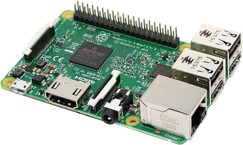
\includegraphics[width=0.3\textwidth]{pictures/raspberry_pi.jpg}
  \captionsetup{justification=centering, labelformat=simple, singlelinecheck=false}
    \caption[Raspberry Pi Model B]{Raspberry Pi Model B\\ Quelle: siehe \cite{raspberry_pi}}
\end{figure} \\ \\
\noindent
\textbf{Logitech Kamera zur Gesichtserkennung} \\ \\
Für die Gesichtserkennung wird eine Logitech Kamera verwendet, die eine hohe Bildqualität und eine zuverlässige Leistung bietet. Diese Kamera ist über USB mit dem Raspberry Pi verbunden und ermöglicht es, Benutzer zu erkennen und auf sie zugeschnittene Informationen anzuzeigen. In der nachfolgenden Abbildung kann die Kamera entnommen werden.\\ \\
\noindent
\begin{figure}[h]
    \centering
    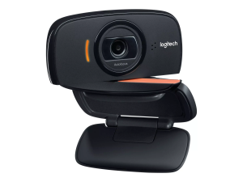
\includegraphics[width=0.3\textwidth]{pictures/logitech_kamera.png}
  \captionsetup{justification=centering, labelformat=simple, singlelinecheck=false}
    \caption[Logitech Kamera]{Logitech Kamera\\ Quelle: siehe \cite{logitech_camera}}
\end{figure} \\ \\
\noindent
\textbf{Monitor} \\ \\
Der Dell 2208WFP Monitor dient als Display für den Smartmirror. Er ist über den integrierten VGA Anschluss mithilfe eines Adapters mit dem Raspberry PI verbunden und ist in das Spiegelgehäuse integriert. Der Monitori wir in der Nachfolgenden Abbildung ersichtlich. \\ \\
\noindent
\begin{figure}[h]
    \centering
    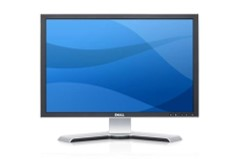
\includegraphics[width=0.3\textwidth]{pictures/dell_monitor.jpg}
  \captionsetup{justification=centering, labelformat=simple, singlelinecheck=false}
    \caption[Dell Monitor]{Dell Monitor\\ Quelle:  siehe \cite{dell_monitor}}
\end{figure} \\ \\
\noindent
\textbf{WLAN Stick} \\ \\
Ein WLAN Stick wird verwendet, um den Raspberry Pi mit dem Internet zu verbinden. Dies ermöglicht die Nutzung von Online-Diensten und die Kommunikation mit anderen Geräten im Netzwerk. Dies ist esentiell um die Funktionsweise des Smart Mirrors zu gewährleisten. \\ \\
\noindent
\textbf{Smartphone} \\ \\
Ein Smartphone dient als mobile Schnittstelle für den Smartmirror. Über eine App können Benutzer Einstellungen vornehmen. Eine genaue beschreibung dieser Schnittstelle erfolgt im Abschnitt (ergänzen). \\ \\
\noindent
\section{Auswahlkriterien}
Die Auswahl der Hardware KOmponenten basierte auf mehrere Kriterien, diese werden nun im folgenden genauer beschrieben:
\begin{itemize}
    \item \textbf{Kompatibilität:} Alle Komponenten mussten kompatibel miteinander und mit der Software-Plattform des Smartmirrors sein.
    \item \textbf{Leistung:} Der Raspberry Pi 3 Model B wurde wegen seiner ausreichenden Rechenleistung und Energieeffizienz gewählt.
    \item \textbf{Bildqualität:} Die Logitech Kamera wurde aufgrund ihrer hohen Auflösung und zuverlässigen Gesichtserkennung ausgewählt.
    \item \textbf{Displayqualität:} Der Dell Monitor bietet eine klare und scharfe Anzeige, was für die visuelle Darstellung der Informationen wichtig ist.
    \item \textbf{Konnektivität:} Der WLAN Stick sorgt für eine stabile Internetverbindung, was für die Nutzung von Online-Diensten unerlässlich ist.
    \item \textbf{Benutzerfreundlichkeit:} Das Smartphone als mobile Schnittstelle erleichtert die Interaktion und die Anpassung der Einstellungen durch den Benutzer.
\end{itemize}
\section{Installation}
In diesem Abschnitt wird nun die einzelnen schritte beachtet, welche bei der installierung der unterschiedlichen Hardware Komponennten vorgegangen sind. \\ \\
\noindent
\textbf{Raspberry Pi 3 Model B}
\begin{itemize}
    \item Die microSD-Karte wurde formatiert und das Betriebssystem wurde darauf installiert.
    \item Der Raspberry Pi wurde in das Gehäuse eingebaut und mit dem Monitor über den VGA auf HDMI Adapter verbunden.
    \item Die Stromversorgung wurde angeschlossen und der Raspberry Pi wurde gestartet.
\end{itemize}
\vspace{0.5cm}
\noindent\textbf{Logitech Kamera}
\begin{itemize}
    \item Die Kamera wurde über USB mit dem Raspberry Pi verbunden.
\end{itemize}
\vspace{0.5cm}
\noindent\textbf{Monitor}
\begin{itemize}
    \item Der Monitor wurde in das Spiegelgehäuse integriert und mit dem Raspberry Pi verbunden.
\end{itemize}
\vspace{0.5cm}
\noindent\textbf{WLAN Stick}
\begin{itemize}
    \item Der WLAN Stick wurde in einen freien USB-Port des Raspberry Pi eingesteckt.
\end{itemize}
\vspace{0.5cm}
\noindent\textbf{Smartphone}
\begin{itemize}
    \item Eine spezielle App wurde auf dem Smartphone installiert, um die Kommunikation mit dem Smartmirror zu ermöglichen.
    \item Das Smartphone wurde mit dem WLAN des Raspberry Pi verbunden
\end{itemize}

\section{Konfiguration}
Ich folgenden Abschnitt wird nun beschrieben wie die unterschiedlichen Hardware Komponenten Konfiguriert wurden. \\ \\
\noindent
\textbf{Raspberry Pi 3 Model B:}
Die Konfiguration des Raspberry Pi umfasste die Installation von den beödigten Software Paketen und das Einrichten von Netzwerkeinstellungen. \\ \\
\noindent
\textbf{Logitech Kamera:}
Die Gesichtserkennungssoftware wurde installiert und entsprechend kalibriert. Desweiteren wurden die Kameraeinstellungen angepasst, um eine optimale Erkennungsrate zu gewährleisten. \\ \\
\noindent
\textbf{Monitor (Dell 2208WFP):}
Die Bildschirmeinstellungen wurden so konfiguriert, dass der Monitor im Energiesparmodus bleibt, wenn der Smartmirror nicht verwendet wird. Des weiteren wurde die Anzeigesoftware für den Smartmirror installiert und konfiguriert. \\ \\
\noindent
\textbf{WLAN Stick:}
Die Netzwerkkonfiguration wurde angepasst, um sicherzustellen, dass der Smartmirror eine stabile Verbindung zum Internet hat. \\ \\
\noindent
\textbf{Smartphone:}
Die App auf dem Smartphone wurde installiert. \\ \\
\noindent


\input{rahmen}

\chapter{Display}

In diesem Kapitel gehen wir auf das Display ein, das im \textbf{Spiegel AI} Projekt verwendet wird. Wir beschreiben die Spezifikationen, die Installation und die Anpassungen, die vorgenommen wurden.

\section{Spezifikationen}
Beschreiben Sie die technischen Spezifikationen des Displays.

\section{Installation}
Erläutern Sie den Prozess der Installation des Displays.

\section{Anpassungen}
Beschreiben Sie etwaige Anpassungen oder Modifikationen am Display.

\subsection{eventuell HTMl seite und Aufbau oder in Installation}

\subsection{Widgets Aktualisierung}
Erarbeitet von: Leon Kranner \\ \\

Alle Widgets müssen in regelmäßiger Zeit aktualisiert werden. Wie regelmäßig dies der Fall ist, hängt vom Widget ab. Dies regelt die Timer.js Datei. Hier werden alle Widgets aktualisiert und die neusten Daten geladen. In diesem Abschnitt ist eine kleine Übersicht wie regelmäßig die Widgets geladen werden: \\

\begin{enumerate}
    \item \textbf{Uhr}
    Jede Sekunde
    
    \item \textbf{Termine:}
    Alle 60 Sekunden
    
    \item \textbf{JKalender:}
    Jeden Tag um Mitternacht
    
    \item \textbf{Wettervorhersage:}
    Alle 3 Stunden
    
    \item \textbf{Tankstellen:}
    Alle 10 Sekunden

 \item \textbf{Tankstellen:}
    Alle 10 Sekunden

 \item \textbf{Verkehrsinformationen:}
    Alle 5 Minuten
\end{enumerate}

\subsection{Termine Widget}
Erarbeitet von: Leon Kranner \\ \\

\noindent
Das Termin-Widget ist eine JavaScript-Anwendung, die dazu dient, die nächsten drei anstehenden Termine auf dem Display anzuzeigen. Dieses Widget filtert die Termine, sortiert sie nach Datum und stellt sicher, dass nur zukünftige Termine angezeigt werden. Die Termine werden dynamisch in eine HTML-Liste eingefügt. \\ \\
In Zukunft soll die App die nächsten Termine aus der Smartphone Kalender App abrufen und den Raspberry versenden. Somit werden die aktuellen Termine automatisch geladen und müssen nicht manuell eingetragen werden.

\begin{figure}[h]
    \centering
    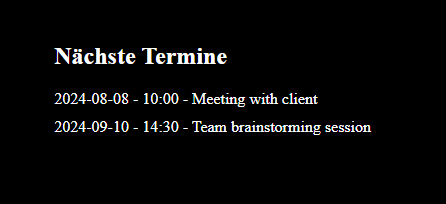
\includegraphics[width=0.4\textwidth]{pictures/appointments_widget.png}
  \captionsetup{justification=centering, labelformat=simple, singlelinecheck=false}
    \caption[Termine Widget]{Termine Widget\\ Quelle: eigene Darstellung}
\end{figure}

\noindent
Die Hauptfunktion des Widgets ist \texttt{loadAppointments()}, die beim Laden der Seite ausgeführt wird. Die Funktion filtert, sortiert und rendert die Termine auf dem Display.

\subsection*{Detaillierte Beschreibung der Funktion \texttt{loadAppointments}}
Die Funktion \texttt{loadAppointments()} führt folgende Schritte aus:

\begin{enumerate}
    \item \textbf{Terminliste initialisieren:}
    Ein Array von Terminen (\texttt{appointments}) wird definiert, das Datum, Uhrzeit und Beschreibung jedes Termins enthält.
    
    \item \textbf{Heutiges Datum ermitteln:}
    Das heutige Datum (\texttt{today}) wird mithilfe des \texttt{Date}-Objekts ermittelt.
    
    \item \textbf{HTML-Elemente vorbereiten:}
    Das HTML-Element mit der ID \texttt{appointmentsList} wird selektiert und dessen Inhalt wird geleert.
    
    \item \textbf{Filtern der zukünftigen Termine:}
    Es werden nur die Termine gefiltert, deren Datum gleich oder später als das heutige Datum ist.
    
    \item \textbf{Sortieren der Termine:}
    Die gefilterten Termine werden nach Datum sortiert.
    
    \item \textbf{Hinzufügen der Termine zur Liste:}
    Für jeden gefilterten und sortierten Termin wird ein \texttt{li}-Element erstellt, das die Termininformationen enthält. Diese \texttt{li}-Elemente werden zur \texttt{appointmentsList} hinzugefügt.
    
    \item \textbf{Seitenladezustand:}
    Die Funktion wird beim ersten mal in der appoinment.js Datei aufgerufen. Da sich Termine jederzeit ändern können, soll in regelmäßigen Abständen das Termin Widget aktualisiert werden.
\end{enumerate}

\noindent
Das Termin-Widget bietet eine einfache und effektive Lösung zur Anzeige bevorstehender Termine. Es lässt sich leicht in bestehende Webseiten integrieren und an individuelle Bedürfnisse anpassen.

\subsection{Kalender Widget}
Erarbeitet von Leon Kranner \\ \\

\noindent
Das Kalender-Widget ist eine JavaScript-Anwendung, die den aktuellen und den nächsten Monat in einem Kalender nebeneinander anzeigt. Der aktuelle Tag wird dabei hervorgehoben. \\

\begin{figure}[h]
    \centering
    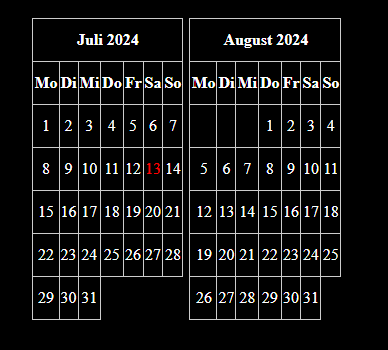
\includegraphics[width=0.5\textwidth]{pictures/calendar_widget.png}
  \captionsetup{justification=centering, labelformat=simple, singlelinecheck=false}
    \caption[Kalender Widget]{Kalender Widget\\ Quelle: eigene Darstellung}
\end{figure}

\noindent
Ursprünglich sollte der aktuelle Tag durch einen roten Ring markiert werden. Jedoch gab es Probleme bei der Formatierung, da die Zahl nicht mittig im Ring angezeigt wurde, sondern unübersichtlich an der Seite des Feldes., Gelöst wurde dieses Problem, in dem wir einen anderen Ansatz probiert haben. Der aktuelle Tag wird jetzt rot markiert und nicht eingekreist.\\
Ein weiteres Problem war die generelle Formatierung des Kalenders: Die Zahlen haben teilweise nicht mit den Wochentag übereingestimmt oder die Tage wurden leicht verschoben und haben nicht mehr gepasst. Außerdem hat der der erste Tag des Monats immer mit einen Montag begonnen. Nach einer längeren Bugfixing-Session und längerer Überarbeitung konnten die Fehler gelöst werden. \\
Zunächst wurden die Monate untereinander angezeigt. Da wir das Programm noch nicht auf dem Raspberry und den Bildschirm übertragen haben, konnten wir noch nicht testen, ob das Layout passt. Beim Testen viel auf, dass der zweite Monat abgeschnitten wurde, weshalb wir uns dazu entschieden haben, die Monate nebeneinander anzuzeigen.

\noindent
Die Hauptfunktion des Widgets ist \texttt{createCalendarWidget()}, die beim Laden der Seite ausgeführt wird. Diese Funktion generiert die Kalender für den aktuellen und den nächsten Monat und zeigt sie in definierten Containern nebeneinander an.

\subsection*{Detaillierte Beschreibung der Funktion \texttt{createCalendarWidget}}
Die Funktion \texttt{createCalendarWidget()} führt folgende Schritte aus:

\begin{enumerate}
    \item \textbf{Elemente vorbereiten:}
    \begin{itemize}
        \item Das HTML-Element mit der ID \texttt{calendarWidget} wird selektiert.
        \item Die HTML-Elemente für den aktuellen Monat (\texttt{currentMonthCalendar}) und den nächsten Monat (\texttt{nextMonthCalendar}) werden selektiert.
    \end{itemize}

    \item \textbf{Kalender generieren:}
    Die Funktion \texttt{generateCalendar()} wird verwendet, um den HTML-Code für die Kalender zu generieren und in die entsprechenden Container einzufügen.
    
    \item \textbf{Kalenderfunktion \texttt{generateCalendar()}:}
    \begin{itemize}
        \item Berechnung des ersten Tages des Monats und Anzahl der Tage im Monat.
        \item Aufbau des HTML-Codes für den Kalender mit den Monats- und Wochentagsnamen.
        \item Hinzufügen der Tage in die Tabelle, wobei der aktuelle Tag rot markiert wird.
    \end{itemize}

    \item \textbf{Anzeige des Kalenders:}
    Die Kalender für den aktuellen Monat und den nächsten Monat werden in den jeweiligen Containern angezeigt.

 \item \textbf{Seitenladezustand:}
    Die Funktion wird beim ersten mal in der Calendar.js Datei aufgerufen. Sollte sich das Profil bzw. der Zustand des Displays nicht ändern, wird jeden Tag um 24 Uhr der Kalender aktualisiert, um den nächsten Tag  bzw. den nächsten Monat anzeigen zu können.
\end{enumerate}

\noindent
Das Kalender-Widget bietet eine einfache und effektive Lösung zur Anzeige der aktuellen und kommenden Monatskalender. Es lässt sich leicht in den Smart Mirror integrieren und an individuelle Bedürfnisse anpassen. Die Hervorhebung des aktuellen Tages erleichtert die Orientierung im Kalender.


\subsection{Wettervorhersage Widget}
Erarbeitet von: Leon Kranner \\ \\

\noindent
Das Wettervorhersage-Widget ist eine JavaScript-Anwendung, die mithilfe der OpenWeatherMap API die Wettervorhersage für die nächsten drei Tage für eine bestimmte Stadt anzeigt. Das Widget lädt die Wetterdaten über eine API und zeigt die Vorhersage für den aktuellen Tag sowie die nächsten zwei Tage an. \\
In Zukunft soll man in der App den Standort auswählen können, damit der Nutzer entweder den Standort des Spiegels angeben kann oder z.B. auch das Wetter bei der OTH Regensburg ansehen können.

\begin{figure}[h]
    \centering
    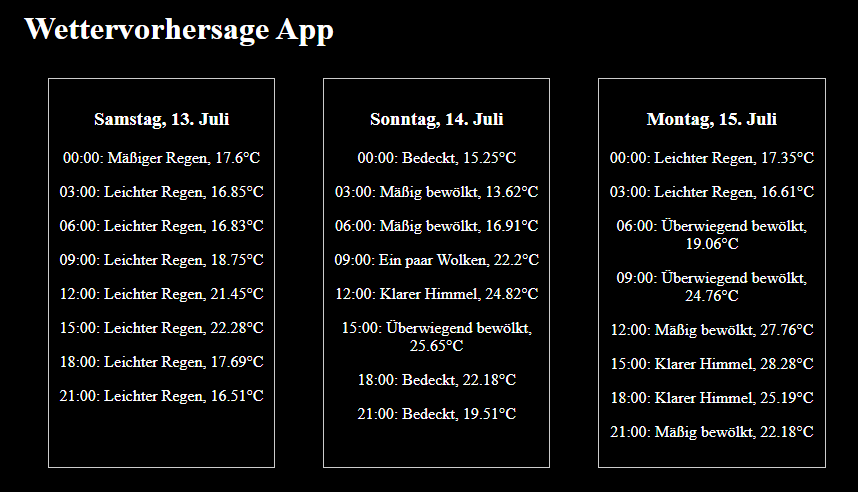
\includegraphics[width=0.4\textwidth]{pictures/forecast_widget.png}
  \captionsetup{justification=centering, labelformat=simple, singlelinecheck=false}
    \caption[Wettervorhersage Widget]{Wettervorhersage Widget\\ Quelle: eigene Darstellung}
\end{figure}

\noindent
Die Hauptfunktionen des Widgets sind \texttt{getForecast()} und \texttt{displayForecast(data)}. \texttt{getForecast()} ruft die Wetterdaten von der API ab, während \texttt{displayForecast(data)} die Daten verarbeitet und auf der Webseite anzeigt.

\subsection*{Detaillierte Beschreibung der Funktion \texttt{getForecast}}
Die Funktion \texttt{getForecast()} führt folgende Schritte aus:

\begin{enumerate}
    \item \textbf{API-Schlüssel und Stadt definieren:}
    Der API-Schlüssel und die Stadt, für die die Wettervorhersage abgerufen werden soll, werden definiert.
    
    \item \textbf{URL für den API-Aufruf erstellen:}
    Eine URL für den API-Aufruf wird mit dem API-Schlüssel und der Stadt erstellt.
    
    \item \textbf{API-Aufruf durchführen:}
    Ein Fetch-Aufruf wird durchgeführt, um die Wetterdaten von der OpenWeatherMap API abzurufen.
    
    \item \textbf{Fehlerbehandlung:}
    Falls die Stadt nicht gefunden wird oder ein anderer Fehler auftritt, wird eine Fehlermeldung angezeigt.
    
    \item \textbf{Daten verarbeiten:}
    Die erhaltenen Daten werden an die Funktion \texttt{displayForecast(data)} übergeben, um sie auf dem Display anzuzeigen.
\end{enumerate}

\subsection*{Detaillierte Beschreibung der Funktion \texttt{displayForecast(data)}}
Die Funktion \texttt{displayForecast(data)} führt folgende Schritte aus:

\begin{enumerate}
    \item \textbf{Vorhersage-Div vorbereiten:}
    Das HTML-Element mit der ID \texttt{forecast} wird selektiert und dessen Inhalt wird geleert.
    
    \item \textbf{Daten nach Tagen gruppieren:}
    Die Wetterdaten werden nach Tagen gruppiert und in einem Objekt gespeichert.
    
    \item \textbf{Vorhersage für drei Tage anzeigen:}
    Es werden nur die Vorhersagen für den aktuellen Tag und die nächsten zwei Tage angezeigt.
    
    \item \textbf{Tagesvorhersagen generieren:}
    Für jeden Tag wird ein Div-Element erstellt, das die Tagesvorhersage enthält. Jede Tagesvorhersage zeigt die Uhrzeit, eine Beschreibung des Wetters und die Temperatur an.
    
    \item \textbf{Vorhersagen in das HTML einfügen:}
    Die generierten Tagesvorhersagen werden in das HTML-Element \texttt{forecast} eingefügt.
\end{enumerate}


\noindent
Das Wettervorhersage-Widget bietet eine einfache und effektive Lösung zur Anzeige der Wettervorhersage für die nächsten drei Tage. Es lässt sich leicht im Display integrieren und an individuelle Bedürfnisse anpassen. Die Nutzung der OpenWeatherMap API ermöglicht eine zuverlässige und aktuelle Wettervorhersage.


\subsection{Notizen Widget}
Erarbeitet von: Leon Kranner \\ \\

\noindent
Das Notizen-Widget ist eine JavaScript-Anwendung, die es dem Benutzer ermöglicht, Notizen zu erstellen und zu speichern. Diese Notizen werden im lokalen Speicher des Browsers gespeichert, sodass sie auch nach dem Schließen des Browsers erhalten bleiben.

\begin{figure}[h]
    \centering
    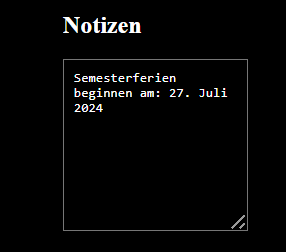
\includegraphics[width=0.4\textwidth]{pictures/notes_widget.png}
  \captionsetup{justification=centering, labelformat=simple, singlelinecheck=false}
    \caption[Notizen Widget]{Notizen Widget\\ Quelle: eigene Darstellung}
\end{figure}

\noindent
Die Hauptfunktionen des Widgets sind \texttt{loadNotes()} und \texttt{saveNotes()}. \texttt{loadNotes()} lädt die gespeicherten Notizen aus dem lokalen Speicher, während \texttt{saveNotes()} die Notizen im lokalen Speicher speichert.

\subsection*{Detaillierte Beschreibung der Funktion \texttt{loadNotes}}
Die Funktion \texttt{loadNotes()} führt folgende Schritte aus:

\begin{enumerate}
    \item \textbf{Gespeicherte Notizen abrufen:}
    Die Notizen werden aus dem lokalen Speicher des Browsers abgerufen.
    
    \item \textbf{Notizen im Textbereich anzeigen:}
    Wenn gespeicherte Notizen vorhanden sind, werden sie im Textbereich (\texttt{notesTextarea}) angezeigt.
\end{enumerate}

\subsection*{Detaillierte Beschreibung der Funktion \texttt{saveNotes}}
Die Funktion \texttt{saveNotes()} führt folgende Schritte aus:

\begin{enumerate}
    \item \textbf{Notizen aus dem Textbereich abrufen:}
    Der Inhalt des Textbereichs (\texttt{notesTextarea}) wird abgerufen.
    
    \item \textbf{Notizen im lokalen Speicher speichern:}
    Die Notizen werden im lokalen Speicher des Browsers gespeichert.
\end{enumerate}

\subsection*{Eventlistener}
Die Anwendung nutzt zwei Eventlistener:

\begin{itemize}
    \item \textbf{\texttt{DOMContentLoaded}-Event:}
    Lädt die Notizen, sobald die Seite vollständig geladen ist.
    
    \item \textbf{\texttt{input}-Event:}
    Speichert die Notizen, sobald der Benutzer den Text ändert.
\end{itemize}

\noindent
Das Notizen-Widget bietet eine einfache und effektive Lösung zur Erstellung und Speicherung von Notizen im lokalen Speicher des Browsers. Es lässt sich leicht in bestehende Webseiten integrieren und an individuelle Bedürfnisse anpassen. Die Nutzung des lokalen Speichers ermöglicht eine persistente Speicherung der Notizen, auch nach dem Schließen des Browsers.


\subsection{Uhrzeit Widget}
Erarbeitet von: Marcel Wagner \\ \\
\noindent
Die Implementierung des Uhrzeit Widgets für den Smart Mirror ist ein wichtiger Schritt zur Verbesserung der Funktionalität und Benutzerfreundlichkeit des Geräts. Ziel dieses Widgets ist es, die aktuelle Uhrzeit exakt und zuverlässig anzuzeigen. Wobei die Anzeige in Echtzeit aktualisiert werden muss, um stets die genaue Uhrzeit widerzuspiegeln. In der Nachfolgenden Abbildung kann das Implementierte Uhrzeit Widget entommen werden.\\ \\

\begin{figure}[h]
    \centering
    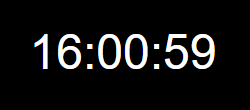
\includegraphics[width=0.4\textwidth]{pictures/time_widget.png}
  \captionsetup{justification=centering, labelformat=simple, singlelinecheck=false}
    \caption[Uhrzeit Widget]{Uhrzeit Widget\\ Quelle: eigene Darstellung}
\end{figure}

\noindent
Die Implementierung des vorher gezeigten Widgets basierte auf der Nutzung von JavaScript zur Echtzeitaktualisierung der Uhrzeit und HTML zur Einbettung des Widgets in die Benutzeroberfläche des Smart Mirrors. Desweiteren wurde CSS benutzt um das Widget zu formatieren. Die JavaScript Funktion sorgt dafür, dass die Uhrzeit jede Sekunde aktualisiert wird, während das HTML Dokument die Struktur definiert. Abschließend definiert die CSS Datei das Styling des Widgets. \\ \\
\noindent
Während der Entwicklung des Widgets traten mehrere Herausforderungen auf. Eine der größten Herausforderungen bestand darin, sicherzustellen, dass die Uhrzeit in Echtzeit und ohne Verzögerung aktualisiert wird. Dies war besonders wichtig, um die Genauigkeit der angezeigten Zeit zu gewährleisten. Die Verwendung der 'setTimeout' Funktion in JavaScript ermöglicht eine wiederholte Ausführung der Aktualisierungsfunktion in einem festgelegten Intervall von einer Sekunde, wodurch eine kontinuierliche und genaue Aktualisierung der Uhrzeit sichergestellt wurde.
Eine weitere Herausforderung war die exakte Zeitanzeige, insbesondere hierbei ist wichtig die Erwähnung der Formatierung der Uhrzeit, um sicherzustellen, dass Stunden, Minuten und Sekunden stets zweistellig angezeigt werden. Durch die Verwendung der 'padStart' Methode konnten die Zahlen auf eine konstante Länge von zwei Stellen gebracht werden, indem bei Bedarf führende Nullen hinzugefügt werden. Dies gewährleistete eine konsistente und gut lesbare Anzeige.\\ \\
\noindent
Das Implementiert Widget wurde im Anschluss auf ihre Funktionalitäten getestet. Auf diesen Bereich wird im Kapitel 3.3.11 genauer für alle Widget eingegangen.


\subsection{Verkehrsinformation}
Erarbeitet von: Marcel Wagner \\ \\
\noindent
Die Implementierung des Stau Widgets auf dem Smart Mirror stellt einen wichtigen Schritt dar, um den Nutzern eine umfassende und zuverlässige Quelle für aktuelle Verkehrsinformationen zur Verfügung zu stellen. Das Widget wurde speziell entwickelt, um eine Echtzeitübersicht über die Verkehrslage in Regensburg zu bieten, was insbesonders für Pendler von großem Nutzen ist. Durch die Verwendung von JavaScript wurde eine nahtlose Integration mit der OpenStreetMap Overpass API realisiert, die als zuverlässige Datenquelle für Verkehrsdaten dient. Bevor die Vrogehensweise der Implementierung betrachtet wird kann der Nachfolgenden Abbildung nun das Implementierte Widget  für dem Fall das aktuelle Kein Stau in Regensburg vorhanden ist entnommen werden. \\ \\
\noindent
\begin{figure}[h]
    \centering
    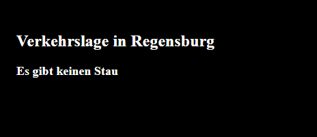
\includegraphics[width=0.4\textwidth]{pictures/traffic_widget.png}
  \captionsetup{justification=centering, labelformat=simple, singlelinecheck=false}
    \caption[Verkehrsinformations Widget]{Verkehrsinformations Widget\\ Quelle: eigene Darstellung}
\end{figure}

\noindent
Die Strategie hinter der Implementierung war zweigleisig: Zum einen wurde eine sofortige Aktualisierung der Verkehrsinformationen beim Laden der Seite implementiert, um den Nutzern bei jedem Besuch des Smart Mirrors die aktuellsten Daten bereitzustellen. Zum anderen erfolgt eine regelmäßige automatische Aktualisierung alle fünf Minuten, um sicherzustellen, dass die angezeigten Informationen kontinuierlich aktuell gehalten werden. Dieser Ansatz gewährleistet eine hohe Aktualität und Relevanz der bereitgestellten Verkehrsinformationen. \\ \\
\noindent
Während der Entwicklung wurden mehrere Herausforderungen gemeistert, darunter die robuste Fehlerbehandlung, um sicherzustellen, dass Netzwerkprobleme oder API Ausfälle die Funktionalität des Widgets nicht beeinträchtigen. Ein besonderes Augenmerk lag auf der Gewährleistung einer stabilen und zuverlässigen Datenaktualisierung, die für eine nahtlose Benutzererfahrung entscheidend ist. \\ \\
\noindent
Das Verkehrs Widget präsentiert die Verkehrslage in einer klaren und intuitiven Benutzeroberfläche. Es informiert die Nutzer klar verständlich darüber, ob derzeit ein Stau vorliegt oder nicht, und bietet gegebenenfalls zusätzliche Informationen über Verkehrshindernisse oder Verkehrswarnungen. Diese klare visuelle Darstellung hilft den Nutzern, schnell zu erfassen, wie die aktuelle Verkehrssituation ihre geplante Route beeinflussen ist. \\ \\
\noindent
Das Implementiert Widget wurde im Anschluss auf ihre Funktionalitäten getestet. Auf diesen Bereich wird im Kapitel 3.3.11 genauer für alle Widget eingegangen.

\subsection{Potenzielle Erweiterungen}
Ein bedeutendes Potenzial für eine Weiterentwicklung des Verkehrs Widgets liegt in der Integration mit der bereits bestehenden Smartphone Schnittstellen, um eine dynamische Anpassung des Standorts zu ermöglichen. Diese Erweiterung würde es den Nutzern gestatten, die Verkehrsinformationen auf ihrem Smart Mirror basierend auf ihrem aktuellen Standort abzurufen. Dies ist besonders relevant für Pendler, die täglich unterschiedliche Routen verwenden oder deren Start- und Zielorte variieren.


\subsection{Schlagzeilen}
Erarbeitet von: Marcel Wagner \\ \\
\noindent
Die Implementierung des Nachrichten Widgets für den Smart Mirror stellt einen wichtigen Schritt dar, um den Nutzern eine aktuelle und relevante Informationsquelle direkt auf seinem Smart Mirror zur Verfügung zu stellen. Das Widget wurde in JavaScript entwickelt und verwendet die 'RSS2JSON-API', um die neuesten Nachrichtenartikel eines ausgewählten RSS Feeds abzurufen und auf dem Smart Mirror anzuzeigen. Dies ermöglicht eine dynamische und automatische Aktualisierung der Nachrichteninhalte, sobald der Nutzer den Spiegel nutzt. In der nachfolgenden Abbildung kann das Funktionierende Widget entnommen werden.\\ \\
\clearpage
\noindent
\begin{figure}[h]
    \centering
    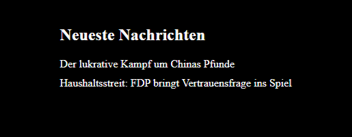
\includegraphics[width=0.4\textwidth]{pictures/news_widget.png}
  \captionsetup{justification=centering, labelformat=simple, singlelinecheck=false}
    \caption[News Widget]{News Widget\\ Quelle: eigene Darstellung}
\end{figure}

\noindent
Ein zentrales Element der Implementierung ist die Verwendung des 'DOMContentLoaded' Events, das sicherstellt, dass das Widget erst aktiv wird, nachdem die gesamte Seite vollständig geladen ist. Dies ist notwendig damit alle notwendigen Ressourcen und Elemente bereitstehen, bevor die Datenabfrage und die Darstellung der Nachrichten beginnen. \\ \\
\noindent
Die Funktionalität des Widgets umfasst die Asynchronität der Datenabfrage über die Fetch API, die die RSS Feeds von Nachrichtenquellen in ein JSON Format umwandelt, das vom JavaScript Code weiterverarbeitet werden kann. Dies ermöglicht eine schnelle und effiziente Bereitstellung der neuesten Nachrichteninhalte direkt auf dem Smart Mirror, ohne dass der Nutzer zusätzliche Schritte unternehmen muss, um sich auf dem Laufenden zu halten. \\ \\
\noindent
Eine besondere Herausforderung während der Implementierung war die unterschiedliche Verfügbarkeit von RSS Feeds bei verschiedenen Nachrichtenseiten. Viele führende Nachrichtenagenturen und Zeitungen bieten zwar RSS Feeds an, einige jedoch nicht oder beschränken den Zugang zu ihren Inhalten über diese Schnittstelle. Dies erforderte eine sorgfältige Auswahl geeigneter RSS Feeds, die eine kontinuierliche und zuverlässige Datenversorgung gewährleisten konnten. Die Ausgegeben Nachrichten dieses Widget sind aus der Frankfurter Allgemeinen Zeitung \\ \\
\noindent
Um die Benutzerfreundlichkeit zu maximieren, wurde die Benutzeroberfläche des Widgets bewusst einfach und intuitiv gestaltet. Die angezeigten Nachrichten werden in einer geordneten Liste präsentiert.
\noindent
Das Implementiert Widget wurde im Anschluss auf ihre Funktionalitäten getestet. Auf diesen Bereich wird im Kapitel 3.3.11 genauer für alle Widget eingegangen.



\subsection{Tankstellen}
Erarbeitet von: Marcel Wagner \\ \\
\noindent
Die Implementierung des Tankstellen Widgets für den Smart Mirror verfolgt das Ziel, den Nutzern eine praktische und zeitnahe Information über den günstigsten Kraftstoffpreise einer Tankstelle in der Nähe zu bieten. Diese Funktionalität wurde durch die Integration von JavaScript und die Nutzung der Tankerkoenig API realisiert, die speziell auf die Abfrage von Tankstellenpreisen und Tankstelleninformationen ausgerichtet ist. In der Nachfolgenden Abbildung kann das Implemntierte Widget entnommen werden. \\ \\
\noindent
\begin{figure}[h]
    \centering
    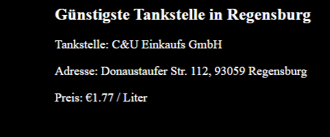
\includegraphics[width=0.4\textwidth]{pictures/gasstation_widget.png}
  \captionsetup{justification=centering, labelformat=simple, singlelinecheck=false}
    \caption[Tankstellen Widget]{Tankstellen Widget\\ Quelle: eigene Darstellung}
\end{figure}

\noindent
Zu Beginn des Implementierungsprozesses wird der 'DOMContentLoaded' Eventlistener verwendet, um sicherzustellen, dass sämtliche Inhalte der Webseite geladen sind, bevor die Datenabfrage gestartet wird. Dies gewährleistet eine stabile und zuverlässige Performance des Widgets auf dem Smart Mirror. Die API Anfrage erfolgt unter Verwendung eines spezifischen API Schlüssels, der die Authentifizierung gegenüber der Tankerkoenig API ermöglicht. Der Standortbezug erfolgt für die Stadt Regensburg mit definierten geografischen Koordinaten. \\ \\
\noindent
Die Datenabfrage wird asynchron durchgeführt, um eine reibungslose Interaktion mit der API zu gewährleisten. Nachdem die Daten abgerufen wurden, erfolgt eine Überprüfung auf erfolgreiche Antwort und die Verfügbarkeit von Tankstelleninformationen. Falls die API Daten erfolgreich zurückgegeben werden und Tankstelleninformationen vorhanden sind, wird die günstigste Tankstelle ermittelt. Dies geschieht durch einen Vergleich der Kraftstoffpreise der abgerufenen Tankstellen, wobei die preisgünstigste Option ausgewählt und deren Informationen weiterverarbeitet werden. \\ \\
\noindent
Die Darstellung der Tankstelleninformationen auf dem Smart Mirror erfolgt in einer klar strukturierten Form. Dies umfasst den Namen der Tankstelle, die vollständige Adresse inklusive Straße, Hausnummer, Postleitzahl und Ort sowie den aktuellen Preis pro Liter Kraftstoff. Diese Informationen sind leicht zugänglich und ermöglichen es dem Nutzer, schnell die wichtigsten Details zu erfassen und eine informierte Entscheidung zu treffen. \\ \\
\noindent
Das Implementiert Widget wurde im Anschluss auf ihre Funktionalitäten getestet. Auf diesen Bereich wird im Kapitel 3.3.11 genauer für alle Widget eingegangen.

\subsection{Potenzielle Erweiterung}
Ein bedeutendes Potenzial für die Weiterentwicklung des Tankstellen-Widgets liegt in der dynamischen Anpassung der Widget Inhalte basierend auf Eingaben vom Smartphone der Nutzer. Diese Erweiterung würde eine noch individuellere und nutzerzentrierte Erfahrung ermöglichen, indem sowohl der bevorzugte Kraftstofftyp als auch der Standort der Nutzer flexibel konfiguriert werden können.

\subsection{Test Verfahren}
Erarbeitet von: Leon Kranner und Marcel Wagner \\ \\
\noindent
Für die implementierten Widgets auf dem Smart Mirror wurden umfangreiche Testverfahren angewendet, die sowohl die Funktionalität als auch die Benutzererfahrung der einzelnen Widgets sicherstellen sollen. Diese unterschiedlichen Testverfahren werden nun im Folgenden genauer beschrieben. \\ \\
\noindent
\textbf{Funktionalitätstests:} Dieser Test konzentrierten sich auf die grundlegenden Aufgaben jedes Widgets. Das Uhrzeitwidget wurde auf seine Fähigkeit getestet, die aktuelle Uhrzeit präzise anzuzeigen. Außerdem wurde sichergestellt, dass die Darstellung formatiert und korrekt aktualisiert wird. Beim News Widget lag der Fokus auf der korrekten Abrufung und Darstellung aktueller Nachrichten, wobei sichergestellt wurde, dass die Informationen stets aktuell und relevant sind. Das Tankstellenwidget durchlief API Integrationstests, um sicherzustellen, dass die Kraftstoffpreise korrekt von der Tankerkoenig API abgerufen und in einem klaren Format angezeigt werden. Das Verkehrsinformations Widget wurde auf seine Fähigkeit geprüft, Verkehrsinformationen zeitnah abzurufen und zuverlässig darzustellen, um Nutzer vor aktuellen Verkehrsbehinderungen zu warnen. \\ \\
\noindent
\textbf{Benutzererfahrungstests:} Diese waren entscheidend, um sicherzustellen, dass die Widgets intuitiv sind. Hierbei halfen Usability Tests, diese bewerteten die Widgets auf Benutzerfreundlichkeit der Benutzeroberfläche. Dabei wurde besonders darauf geachtet, dass die Widgets übersichtlich gestaltet sind und Nutzer schnell die benötigten Informationen finden können. \\ \\
\noindent
\textbf{Performance- und Lasttests:} Diese Testverfahren waren ebenfalls Teil der Teststrategie, um sicherzustellen, dass die Widgets unter verschiedenen Bedingungen effizient arbeiten. Ladezeittests wurden durchgeführt, um sicherzustellen, dass die Widgets schnell genug reagieren und Daten effizient verarbeiten. Skalierbarkeitstests wurden genutzt, um sicherzustellen, dass die Widgets auch bei erhöhtem Datenverkehr stabil bleiben und keine übermäßigen Ressourcen verbrauchen, was besonders wichtig für die Langzeitnutzung ist. \\ \\
\noindent
\textbf{Integrationstest:} Dabei wurden Kompatibilitätstests durchgeführt, um sicherzustellen, dass die Widgets reibungslos mit anderen Komponenten des Smart Mirrors interagieren. Systemtests prüften die Gesamtfunktionalität des Smart Mirrors unter verschiedenen Betriebsbedingungen, um sicherzustellen, dass alle Widgets harmonisch zusammenarbeiten und die Gesamtleistung des Systems nicht beeinträchtigen werden. \\ \\
\noindent
Diese umfassenden Testverfahren stellen sicher, dass die implementierten Widgets nicht nur funktional sind, sondern auch eine qualitativ hochwertige Benutzererfahrung bieten und unter allen Bedingungen zuverlässig arbeiten.





\chapter{Spiegel AI Remote}
\textit{Erarbeitet von David Vollmer.} \\ \\
Im folgenden wird die \textbf{Spiegel AI Remote} App - auch \textbf{Remote App} genannt - beschrieben. Es handelt sich dabei um eine mobile Anwendung, dessen Hauptaufgabe die Fernsteuerung des Smart Mirrors ist.

\section{Die Flutter\texttrademark{} SDK}
Für die Entwicklung einer mobilen Applikation gibt es heutzutage viele Tool-Kits, die verwendet werden können.
\begin{figure}[ht]
    \centering
    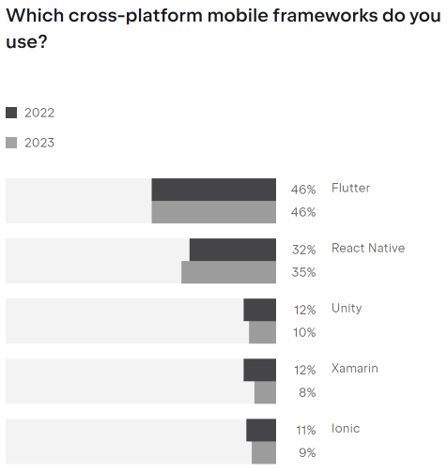
\includegraphics[width=0.4\textwidth]{pictures/frameworks_stats.png}
    \captionsetup{justification=centering, labelformat=simple, singlelinecheck=false}
    \caption{Laut dieser von JetBrains durchgeführten Umfrage war Flutter im Jahr 2023 das am häufigsten verwendete mobile, plattformübergreifende Framework.\cite{jetbrains_survey}}
    \label{fig:jetbrains_survey}
\end{figure} \\
Zusätzlich zu ihrer Popularität ist die von Google entwickelte Flutter SDK in der Lage, mittels AOT-Compiler Programme direkt für die Zielplattform zu kompilieren. Dabei wird die Programmiersprache Dart verwendet.\cite{dart_platform} Flutter unterstützt unter anderem die Entwicklung auf den Plattformen Android SDK, iOS, Windows, macOS und Web.\cite{flutter_supported_platforms} Für die Umsetzung der Fernsteuerungs-App wurde insbesondere mit den Plattformen Android und iOS entwickelt und getestet.

\section{Funktionen}
Um das Display des Spiegel AIs fernzusteuern, müssen einige Hauptfunktionalitäten vorhanden sein. Die Remote App muss in der Lage sein, mit dem Spiegel zu kommunizieren, die Anzeige der Widgets auf dem Display zu ändern, verfügbare Widgets auszuwählen und Profile zu verwalten. Mit Ausnahme der ersten Anforderung, welche im Kapitel \textbf{Schnittstelle} näher beschrieben wird, werden all diese Punkte in sogenannten Ansichten (englisch: views) behandelt. Diese kann der Nutzer mithilfe einer Navigationsleiste auswählen.
\begin{figure}[h]
    \centering
    \begin{minipage}[b]{0.27\textwidth}
        \centering
        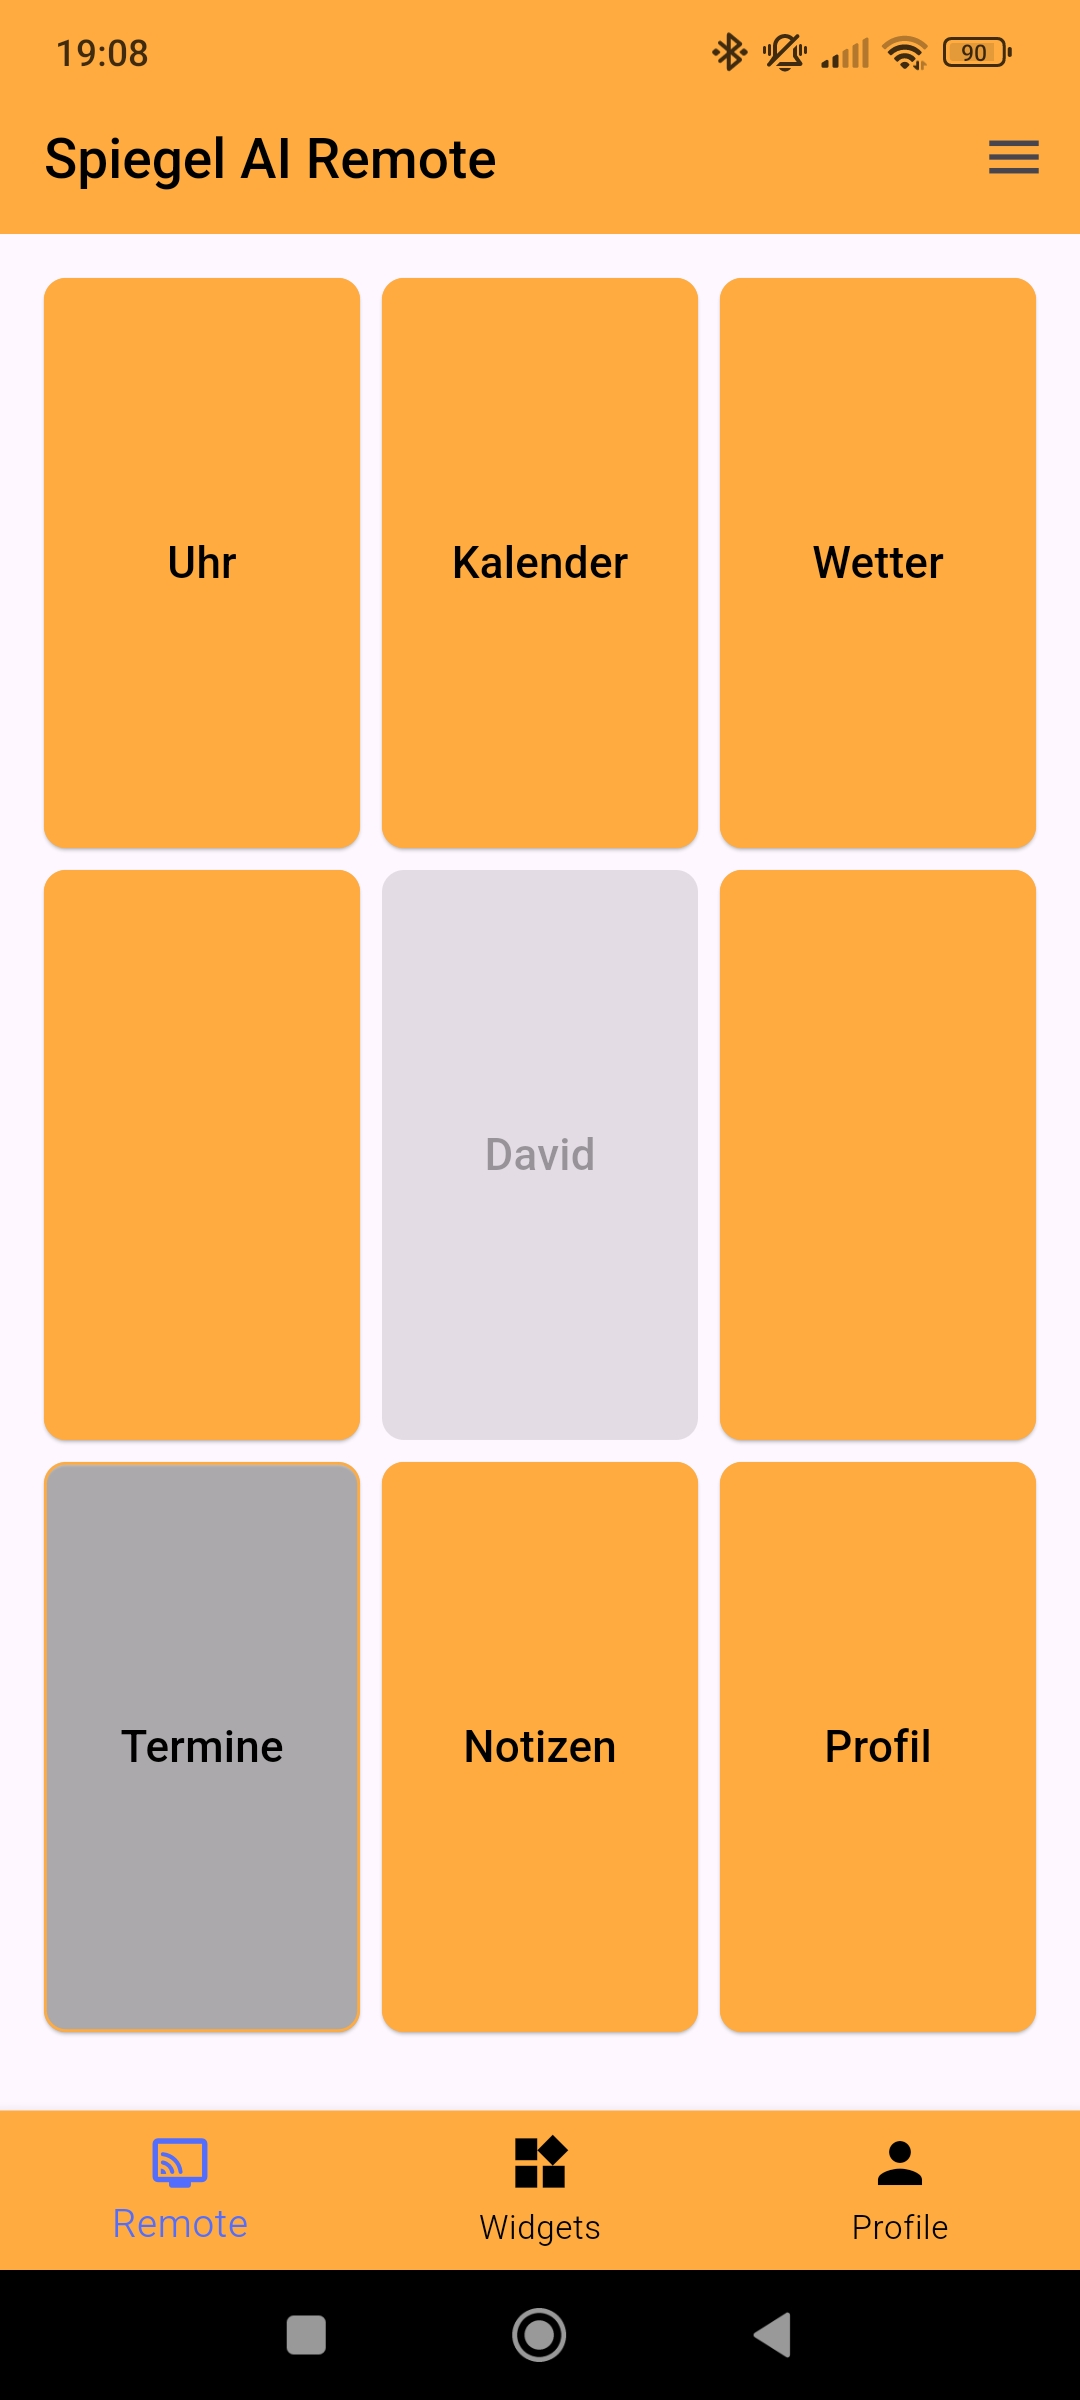
\includegraphics[width=\textwidth]{pictures/remote_remote.jpg}
        \captionsetup{justification=centering, labelformat=simple, singlelinecheck=false}
        \caption{Remote Ansicht}
    \end{minipage}
    \hfill
    \begin{minipage}[b]{0.27\textwidth}
        \centering
        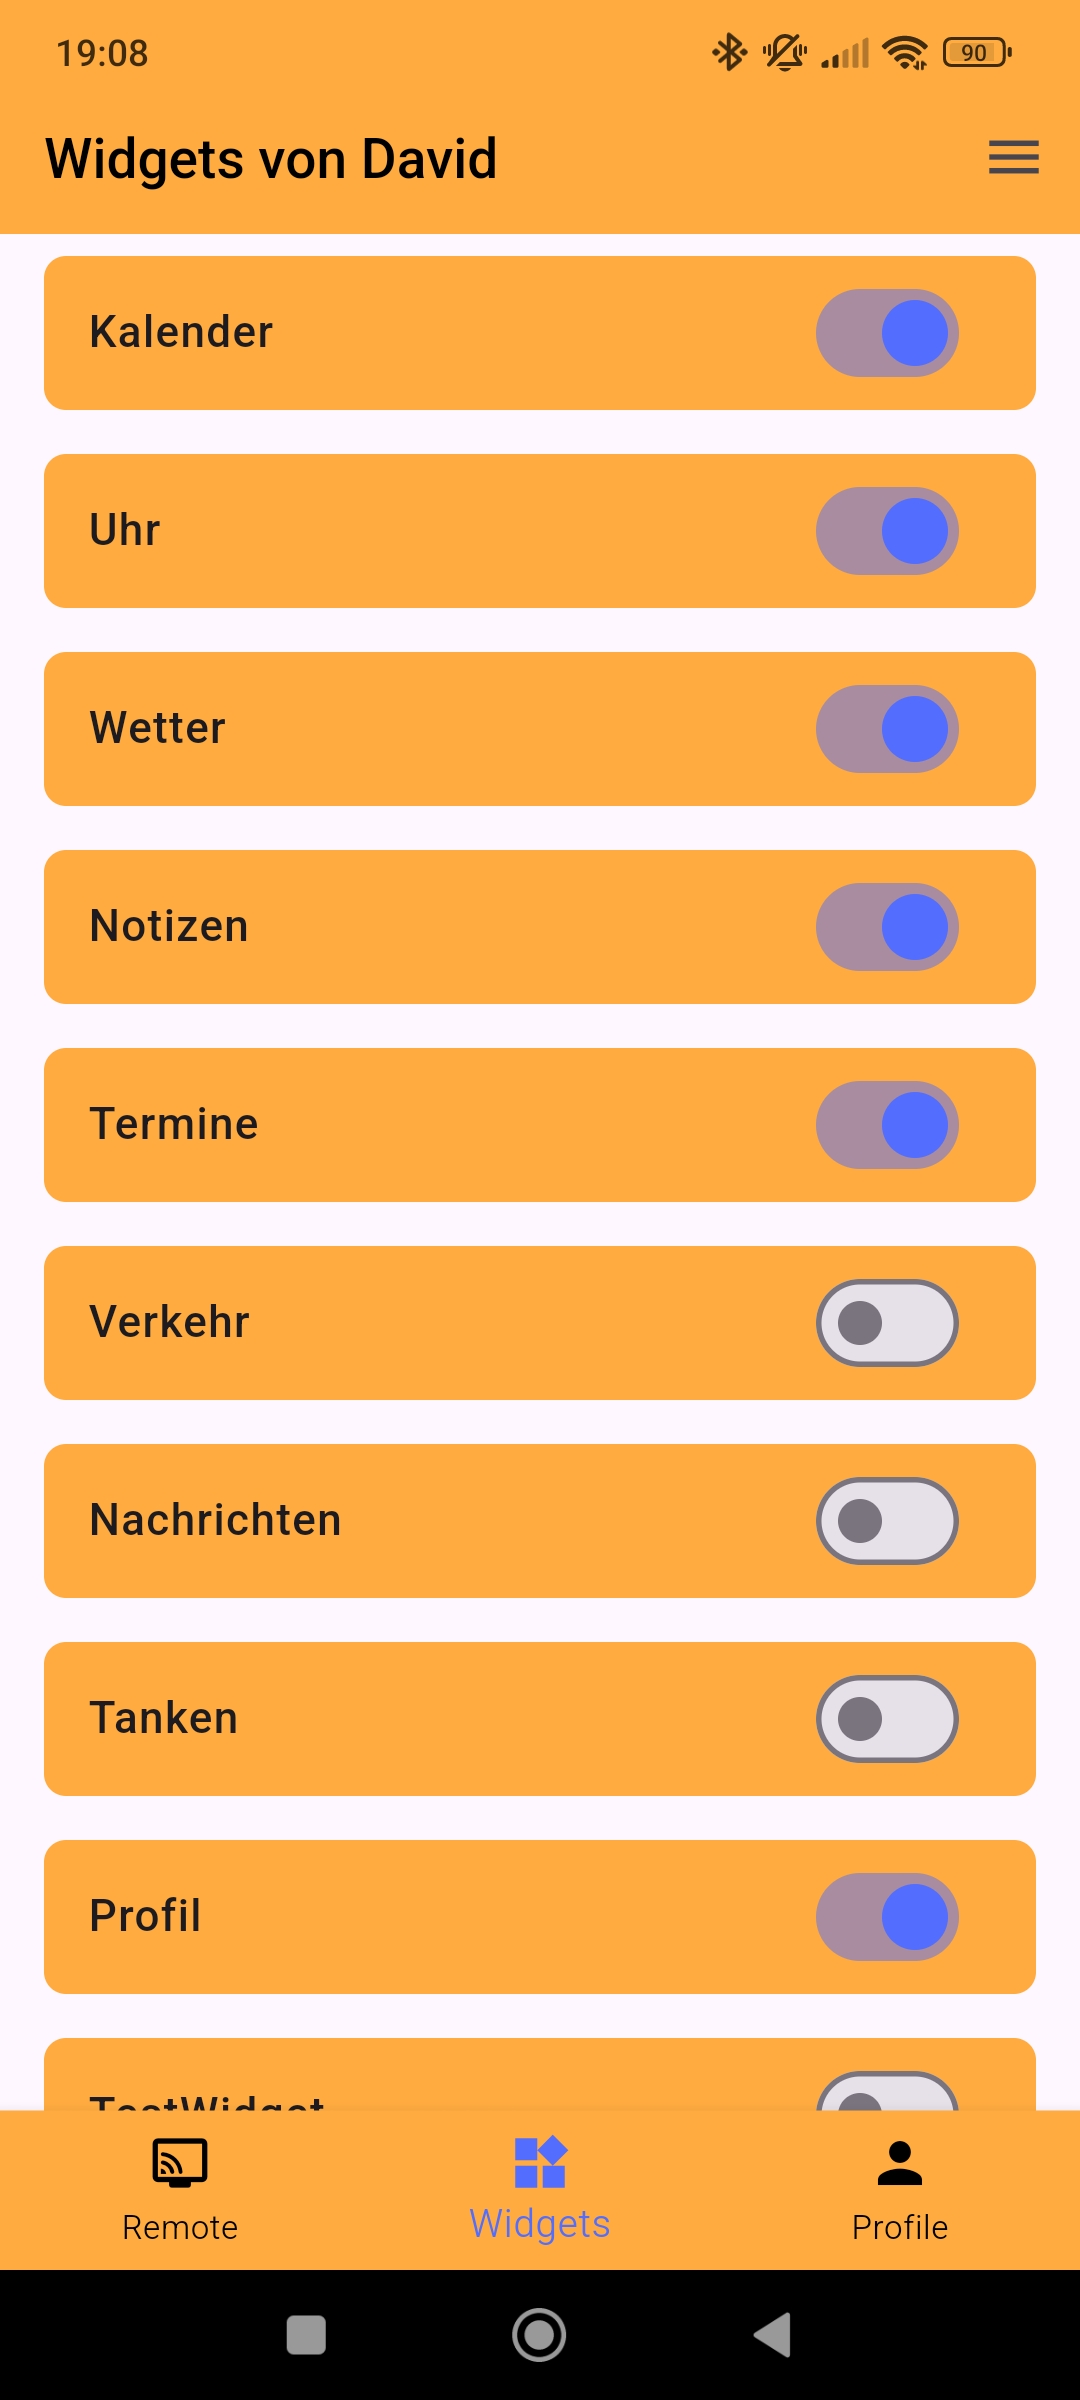
\includegraphics[width=\textwidth]{pictures/remote_widgets.jpg}
        \captionsetup{justification=centering, labelformat=simple, singlelinecheck=false}
        \caption{Widgets Ansicht}
    \end{minipage}
    \hfill
    \begin{minipage}[b]{0.27\textwidth}
        \centering
        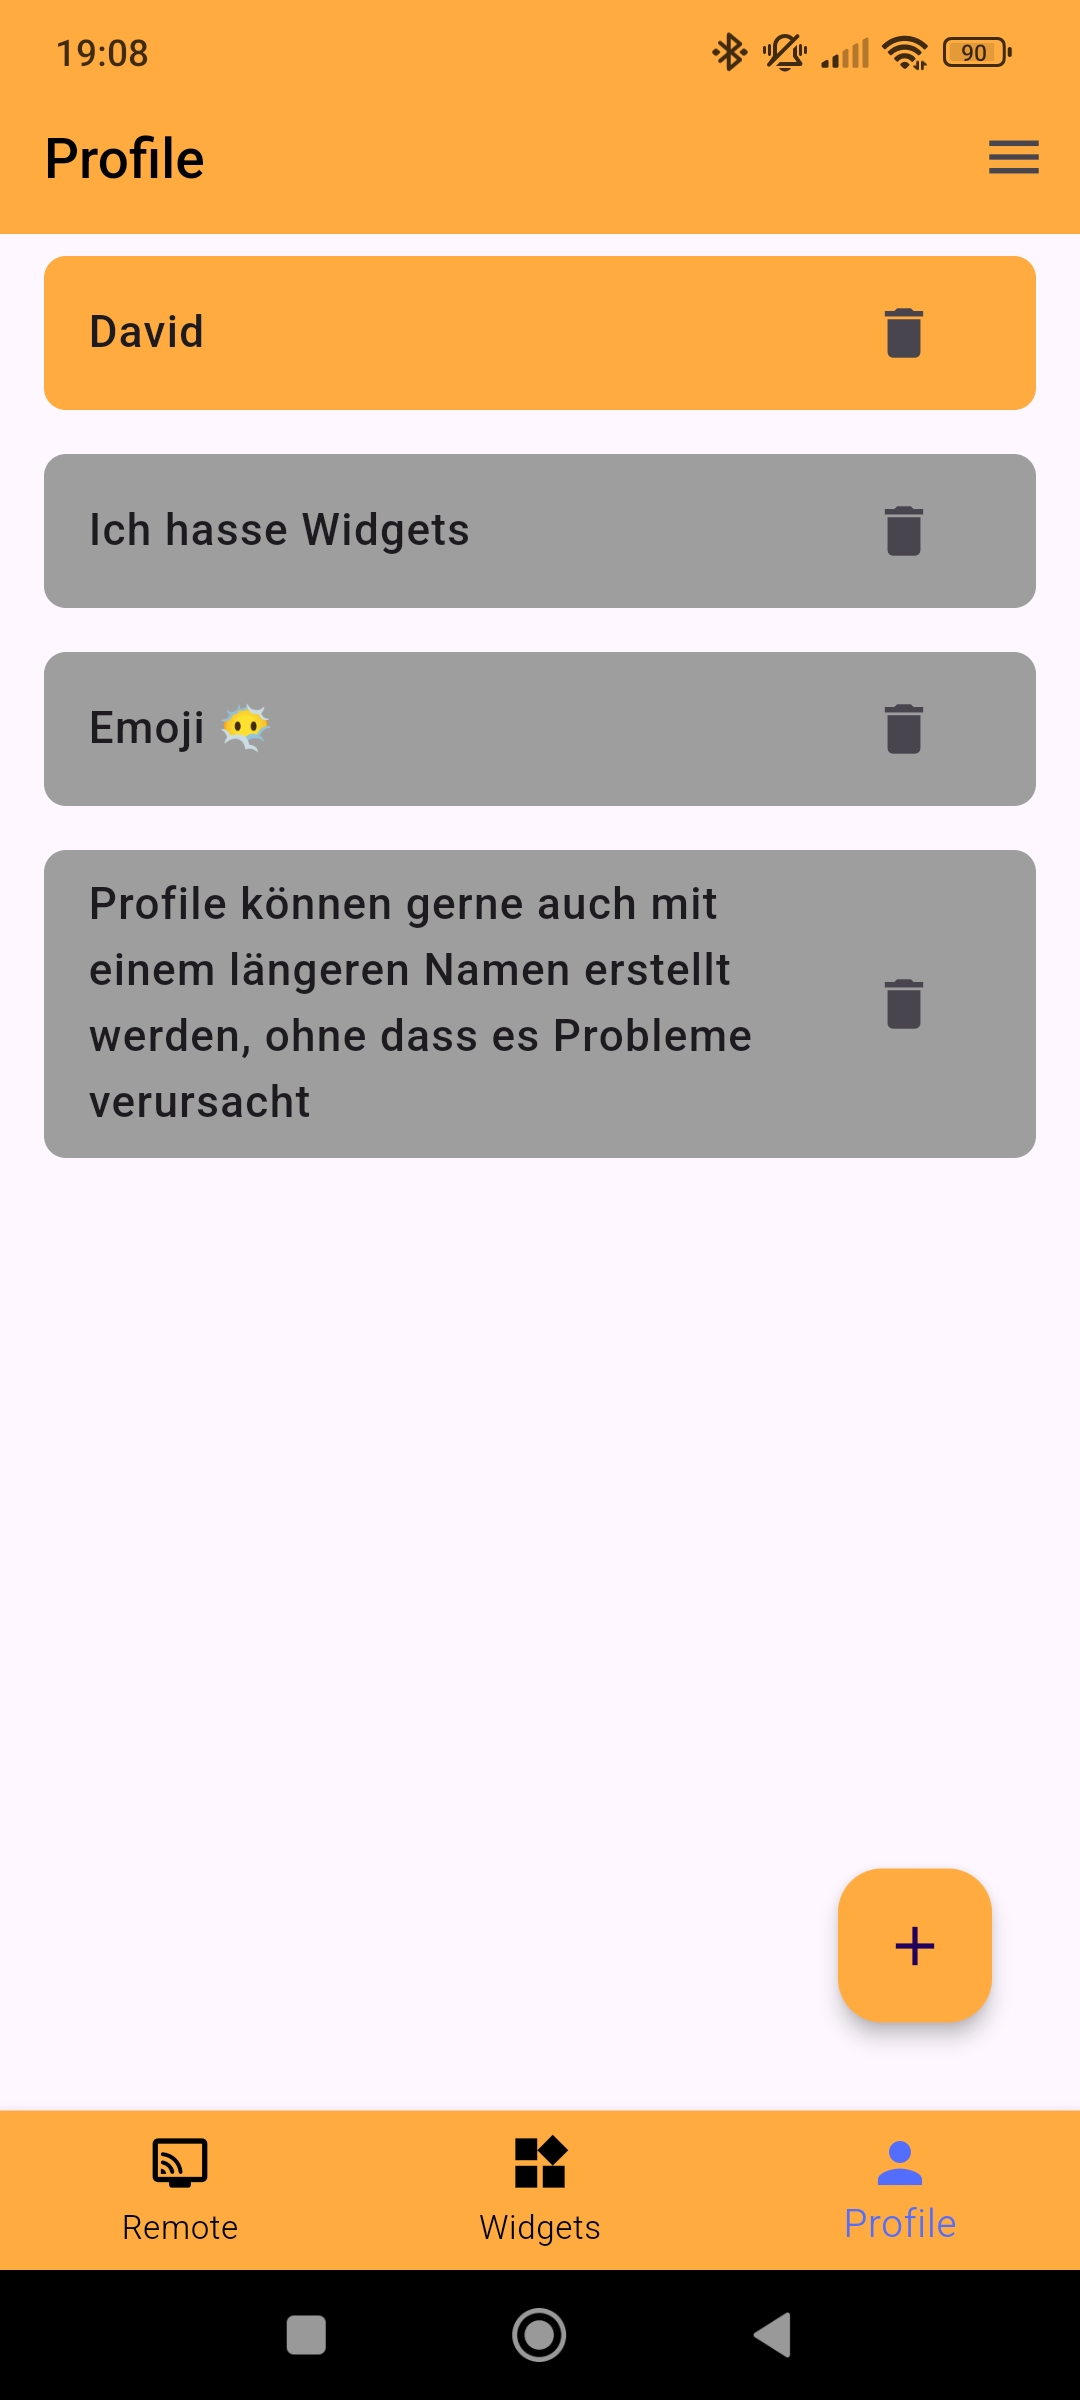
\includegraphics[width=\textwidth]{pictures/remote_profile.jpg}
        \captionsetup{justification=centering, labelformat=simple, singlelinecheck=false}
        \caption{Profile Ansicht}
    \end{minipage}
\end{figure}

\subsection{Remote View}
Die Remote View, welche die Standardansicht nach Öffnen der App ist, bietet die Möglichkeit, den Status der Displayanzeige am Spiegel zu ändern. In der Mitte wird der Name des gerade ausgewählten Profils angezeigt. Dieses Feld lässt keinerlei Interaktion zu, da das zentrale Feld der Spiegelanzeige frei bleibt. Das bedeutet, dass bis zu acht Widgets angezeigt und geändert werden können. Mit einem Klick auf einen Button wird das jeweilige Widget aus- oder eingeblendet. Ein Feld in grauer Farbe bedeutet, dass das Widget vom Spiegel AI Display nicht angezeigt wird. Zieht man ein Widget über ein anderes, werden ihre Positionen getauscht. Die Felder, die keinen Text enthalten, haben die selben Interaktionsmöglichkeiten wie die anderen. Sie sind Platzhalter für Widgets, die hinzugefügt werden können. Falls kein Profil ausgewählt ist, wird im Remote View eine Standardeinstellung angezeigt und jegliche Interaktion der Buttons ist ausgestellt. Bei einem Versuch, ohne Profilselektion eine Änderung vorzunehmen, wird eine Snackbar angezeigt, welche darauf verweist, dass ein Profil geladen sein muss.

\subsection{Widgets View}
In der Widgets Ansicht können für das ausgewählte Profil Widgets ausgewählt werden. Diese View bietet die Widgets Kalender, Uhr, Wetter, Notizen, Termine, Verkehr, Nachrichten, Tanken, Profil und TestWidget an. Bei letzterem handelt es sich um einen Platzhalter, welcher zum Testen der Widgetfunktionalitäten verwendet wurde, aber auch zukünftig mit einem neuen Widget ersetzt werden kann. Die Anwendungen der restlichen Widgets sind im Kapitel \textbf{Display} beschrieben. Mithilfe eines Toggle-Buttons werden bis zu acht Widgets selektiert. Beim Versuch, ein neuntes Widget auszuwählen, schlägt dies fehl und eine Snackbar benachrichtigt über die Obergrenze erlaubter Widgets. Auf die Änderung eines Widgets, ohne ein Profil geladen zu haben, folgt ebenfalls eine dementsprechende Fehlermeldung. Wird ansonsten ein Widget ausgeschaltet, dann wird das im Toggle-Button signalisiert und in der Remote View wird der Name des Widgets mit einem leeren Feld ersetzt. Wenn ein ausgeschaltetes Widget ausgewählt wird, aktualisiert sich auch da der Toggle-Schalter und in der Remote Ansicht wird das erste Feld ohne Textinhalt mit dem Namen des Widgets versehen.

\subsection{Profile View}
Die letzte navigierbare Ansicht ist die Profile View. Hier findet die Verwaltung der gespeicherten Profile statt. Die Profile werden aufgelistet und können mit einem Klick ausgewählt werden. Hält man ein Profil für eine kurze Zeit gedrückt, kann man diese in ihrer Position in der Auflistung ändern, indem man sie an die gewünschte Stelle zieht. Löschen kann man einen Eintrag, indem auf das Mülleimer-Icon geklickt wird. Darauf öffnet sich ein sogenanntes Alert-Dialog, welches das Abbrechen oder Bestätigen der Löschung durchführt. Ein neues Profil kann erstellt werden, indem auf ein Button, welches sich in der Ansicht rechts unten befindet und mit einem '+'-Symbol gekennzeichnet ist, gedrückt wird. Es erscheint ebenfalls ein Alert-Dialog, welches mithilfe eines Texteingabefeldes einen Profilnamen geben kann. Dieser Prozess kann auch abgebrochen oder bestätigt werden. Falls bei Bestätigung der Name des Profils leer oder schon vergeben ist, wird unterhalb des Textfeldes eine entsprechende Fehlermeldung ausgegeben. Wenn das Erstellen des Profils erfolgreich ist, wird das neue Profil direkt ausgewählt und bekommt die ersten acht Widgets in der Widgets View zugeordnet. Sie werden dementsprechend in der Remote Ansicht angezeigt. Alle Anpassungen, die in diesen beiden Ansichten getätigt werden, werden in den jeweilig ausgewählten Profilen gespeichert.

\section{Implementierung}


\section{Testen}
Testen

\chapter{Gesichtserkennung}
\textit{Erarbeitet von Marco Kuner.} \\

\noindent
Diese Dokumentation beschreibt die Entwicklung einer Gesichtserkennungslösung für einen Smart Mirror. Das Projekt wurde im Rahmen eines Vier-Personen-Teams durchgeführt und beinhaltet die Recherche, Implementierung und Optimierung verschiedener Gesichtserkennungstechnologien. Besonderes Augenmerk liegt auf der genauen Protokollierung der Entscheidungsprozesse und der technischen Herausforderungen.

\section{Einleitung}

\subsection{Projektziel}
Das Hauptziel dieses Projekts war die Entwicklung einer fortschrittlichen Gesichtserkennungslösung für einen Smart Mirror. Dieser Smart Mirror sollte in der Lage sein, Benutzer anhand ihrer Gesichter zu erkennen und personalisierte Informationen anzuzeigen. Die Gesichtserkennung sollte zuverlässig unter verschiedenen Bedingungen wie wechselnden Lichtverhältnissen und unterschiedlichen Gesichtswinkeln funktionieren.

\subsection{Bedeutung der Gesichtserkennung}
Gesichtserkennungstechnologien haben in den letzten Jahren erheblich an Bedeutung gewonnen. Sie finden Anwendungen in zahlreichen Bereichen wie Sicherheit, wo sie zur Zugangskontrolle und Überwachung eingesetzt werden, in der Personalisierung, wo sie individuelle Benutzererlebnisse ermöglichen, und in der Benutzerfreundlichkeit, da sie eine nahtlose Interaktion mit technischen Geräten bieten. Die Entwicklung einer zuverlässigen Gesichtserkennung für den Smart Mirror ist also zwingend erforderlich für eine reibungslose Kundenerfahrung.



\section{Recherche und Anfangsphase}

\subsection{Grundlagen der Gesichtserkennung}
Gesichtserkennung ist ein Bereich der Computer Vision, der sich mit der Identifikation von Individuen anhand ihrer Gesichtszüge beschäftigt. Dies geschieht durch den Einsatz von Algorithmen, die charakteristische Merkmale eines Gesichts extrahieren und analysieren. Traditionelle Methoden der Gesichtserkennung umfassen Ansätze wie die Verwendung von Haar-Cascades, während moderne Methoden oft auf tiefen neuronalen Netzwerken basieren.

\subsection{Vergleich von Methoden}
In der Anfangsphase des Projekts wurde zunächst die Möglichkeit in Betracht gezogen, ein eigenes Deep-Learning-Modell für die Gesichtserkennung zu trainieren. Nach weiterer Recherche und intensiver Absprache mit Kommilitonen aus dem KI-Studiengang wurde jedoch festgestellt, dass das Training eines eigenen Modells aufgrund des hohen Zeitaufwands und der benötigten Rechenressourcen nicht praktikabel wäre.

\noindent Daraufhin wurde eine umfassende Recherche zu verschiedenen existierenden Methoden der Gesichtserkennung durchgeführt. Dabei wurden herkömmliche Ansätze wie Haar-Cascades und moderne Ansätze wie Deep Learning verglichen. Haar-Cascades, die auf der Viola-Jones-Methode basieren, bieten den Vorteil einer schnellen Berechnung und einfachen Implementierung, sind jedoch in ihrer Genauigkeit und Robustheit begrenzt. Im Gegensatz dazu bieten moderne Deep-Learning-Ansätze, wie sie in der Dlib-Bibliothek verwendet werden, eine höhere Genauigkeit und Robustheit, erfordern jedoch mehr Rechenleistung und sind komplexer in der Implementierung.



\section{Erste Implementierung mit Haar-Cascades}

\subsection{Haar-Cascade-Ansatz}
Aufgrund des begrenzten Speichers unseres Raspberry Pi wurde zunächst der Haar-Cascade-Ansatz gewählt, da dieser deutlich weniger komplex aufgebaut ist und weniger Rechenleistung erfordert. Haar-Cascades basieren auf der Viola-Jones-Methode, die einen robusten Algorithmus zur Gesichtserkennung darstellt. 

\noindent Die Haar-Cascade-Methode verwendet eine Kaskade von sogenannten Haar-ähnlichen Merkmalen\cite{haar_quelle}. Eine Kaskade in diesem Kontext bedeutet eine Abfolge von Klassifikatoren, die nacheinander angewendet werden, um die Erkennungsgenauigkeit zu erhöhen und gleichzeitig die Rechenleistung zu optimieren. Diese Merkmale sind einfache Muster, die in unterschiedlichen Größen und Positionen auf das Bild angewendet werden, um Kontraste zu erkennen, die typisch für Gesichtszüge sind. \\ \\

\begin{figure}[h!]
    \centering
    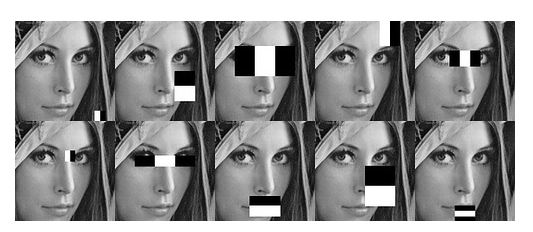
\includegraphics[width=0.5\textwidth]{pictures/haarcascades.jpg}
    \caption{Beispiel verschiedener Haar-ähnlicher Merkmale}
    \label{fig:haar_cascade_example}
    \cite{haar_cascade_example}
\end{figure} 

\noindent Ein integrales Bild wird verwendet, um diese Merkmale effizient zu berechnen. Die Viola-Jones-Methode besteht aus mehreren Hauptkomponenten:\\

\noindent \textbf{Merkmalserkennung}: Haar-ähnliche Merkmale bestehen aus einfachen rechteckigen Bereichen, die Intensitätsunterschiede innerhalb des Bildes messen. Es gibt drei Arten von Haar-ähnlichen Merkmalen: Kantenmerkmale, Linienmerkmale und vierrechteckige Merkmale. Diese Merkmale helfen dabei, grundlegende Strukturen wie Kanten, Linien und Ecken zu erfassen, die in Gesichtern häufig vorkommen. \\

\noindent \textbf{Integralbild}: Das Integralbild ist eine Datenstruktur, die verwendet wird, um die Berechnung von Rechteckmerkmalen in konstanter Zeit zu ermöglichen. Dies wird erreicht, indem für jedes Pixel die Summe aller Pixelwerte oben und links davon berechnet wird. Dadurch kann jedes Rechteckmerkmal durch wenige Zugriffe auf das Integralbild effizient berechnet werden. \\

\noindent \textbf{Adaboost-Training}: Um die Merkmale zu einem starken Klassifikator zu kombinieren, wird der Adaboost-Algorithmus verwendet. Adaboost ist eine Methode des maschinellen Lernens, die eine große Anzahl schwacher Klassifikatoren zu einem starken Klassifikator kombiniert. Während des Trainingsprozesses werden die wichtigsten Merkmale ausgewählt und gewichtet, um die Erkennungsrate zu maximieren und gleichzeitig die Fehlerrate zu minimieren.\\

\noindent \textbf{Kaskadenklassifikation}: Die Klassifikatoren werden in einer Kaskade organisiert, wobei jeder Klassifikator die Aufgabe hat, ein Fenster entweder als Gesicht oder Nicht-Gesicht zu klassifizieren. Ein Fenster, das von einem Klassifikator als Nicht-Gesicht klassifiziert wird, wird sofort verworfen, was die Berechnungen erheblich beschleunigt. Nur Fenster, die von allen Klassifikatoren in der Kaskade als Gesicht erkannt werden, werden letztendlich als Gesicht klassifiziert.\\

\noindent Die ersten Versuche konzentrierten sich darauf, Gesichter in verschiedenen Beleuchtungssituationen und Winkeln zu erkennen, um die Robustheit des Ansatzes zu testen.


\subsection{Vorteile und Nachteile}
Nach der Implementierung des Haar-Cascade-Ansatzes in OpenCV wurde die Methode intensiv getestet, um ihre Vor- und Nachteile zu ermitteln: \\

\noindent \textbf{Vorteile}:
\begin{itemize}
    \item \textbf{Schnelle Berechnung}: Die Methode ist sehr effizient in der Berechnung und kann in Echtzeit auf Geräten mit begrenzten Ressourcen wie dem Raspberry Pi ausgeführt werden.
    \item \textbf{Einfache Implementierung}: OpenCV bietet vorgefertigte Haar-Cascade-Modelle, die leicht zu integrieren sind.
\end{itemize}

\noindent \textbf{Nachteile}:
\begin{itemize}
    \item \textbf{Begrenzte Genauigkeit}: Die Genauigkeit der Erkennung ist begrenzt, insbesondere bei schwierigen Lichtverhältnissen oder seitlich aufgenommenen Gesichtern.
\end{itemize}

\subsection{Ergebnisse der Tests}

 Der Problem lag in der mangelhaften Genauigkeit, insbesondere bei schwierigen Lichtverhältnissen oder seitlich aufgenommenen Gesichtern. Diese Einschränkung lässt sich dadurch erklären, dass Haar-Cascades stark auf Kontraste und einfache geometrische Merkmale angewiesen sind. Bei wechselnden Lichtverhältnissen ändern sich die Intensitätsunterschiede im Bild, was dazu führt, dass die Merkmale, die für die Erkennung verwendet werden, weniger zuverlässig sind. Dies beeinträchtigt die Genauigkeit der Erkennung erheblich, da die Algorithmen Schwierigkeiten haben, die relevanten Merkmale konsistent zu identifizieren.

\noindent Zusammenfassend zeigte sich, dass die Haar-Cascade-Methode zwar effizient in der Berechnung ist und schnell auf Geräten mit begrenzten Ressourcen wie dem Raspberry Pi ausgeführt werden kann, jedoch nicht die erforderliche Präzision und Robustheit für die Gesichtserkennung in einem Smart Mirror bietet. Diese Erkenntnisse führten zur Entscheidung, nach präziseren Methoden für die Gesichtserkennung zu suchen.




\section{Umstieg auf Dlib für höhere Präzision}

\subsection{Wechsel zu Dlib}
Nach dem begrenzten Erfolg mit Haar-Cascades wurde entschieden, auf die Dlib-Bibliothek umzusteigen, um eine robustere Gesichtserkennung zu erreichen. Dlib ist eine freie Software-Bibliothek, die Algorithmen für maschinelles Lernen, Bildverarbeitung und maschinelles Sehen bereitstellt. Für die Gesichtserkennung in diesem Projekt wurde insbesondere der Histogram of Oriented Gradients (HOG)-Algorithmus und das 68-Facial-Landmarks-Modell zur präzisen Merkmalsextraktion verwendet.

\subsection{Technologien: HOG und 68-Facial-Landmarks}
\textbf{Histogram of Oriented Gradients (HOG)}: Der HOG-Algorithmus ist eine Methode zur Merkmalserkennung in Bildern, die darauf basiert, das lokale Auftreten von Gradientenorientierungen zu zählen. Der HOG-Algorithmus bildet die Basis des vortrainierten 68-facial-landsmarks-Modells. Diese Methode funktioniert folgendermaßen:

\begin{itemize}
    \item \textbf{Gradientenberechnung}: Für jedes Pixel im Bild wird der Gradient berechnet. Der Gradient eines Pixels gibt die Richtung und die Stärke der größten Helligkeitsänderung an\cite{hog_quelle}. Dies geschieht durch die Anwendung von Sobel-Filtern in horizontaler und vertikaler Richtung, wodurch zwei Bilder entstehen, die die Helligkeitsänderungen in x- und y-Richtung darstellen. Der Gradient kann dann durch die Kombination dieser beiden Bilder berechnet werden.
    
    \item \textbf{Zellaufteilung}: Das Bild wird in kleine Zellen unterteilt, typischerweise von 8x8 Pixeln. Diese Zellen sind klein genug, um lokale Details zu erfassen, aber groß genug, um signifikante Informationen zu enthalten. Innerhalb jeder Zelle werden die Gradientenorientierungen der Pixel gesammelt und analysiert.
    
    \item \textbf{Orientierungshistogramme}: Für jede Zelle wird ein Histogramm der Gradientenorientierungen erstellt. Die Gradienten innerhalb jeder Zelle werden in Bins sortiert, die verschiedene Richtungen repräsentieren, üblicherweise in 9 Bins, die Winkelbereiche von 0 bis 180 Grad abdecken. Jeder Bin enthält die Summe der Gradientenstärken, die in seine Richtung fallen, was eine robuste Darstellung der Orientierungsmuster innerhalb der Zelle ermöglicht.
    
    \item \textbf{Normierung}: Um die Beleuchtungsunterschiede zu kompensieren, werden die Histogramme in Blöcken normalisiert. Ein Block besteht aus mehreren benachbarten Zellen, typischerweise 2x2. Die Normierung erfolgt durch Berechnung der Quadratwurzel der Summe der quadrierten Bin-Werte, was eine gleichmäßige Darstellung der Merkmale ermöglicht, unabhängig von lokalen Beleuchtungsunterschieden.
    
    \item \textbf{Merkmalsvektor}: Die normalisierten Histogramme aller Blöcke werden zu einem einzigen Merkmalsvektor zusammengefügt, der das Bild repräsentiert. Dieser Merkmalsvektor ist hochdimensional und enthält eine detaillierte Beschreibung der Gradientenorientierungen im gesamten Bild. Er dient als Eingabe für maschinelle Lernalgorithmen, die darauf trainiert sind, Gesichter von Nicht-Gesichtern zu unterscheiden.
\end{itemize}

\begin{figure}[h!]
    \centering
    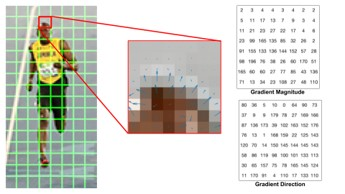
\includegraphics[width=0.5\textwidth]{pictures/hog.jpg}
    \caption{Beispiel einer HOG-Analyse}
    \label{fig:hoganalysis}
    \cite{hoganalysis}
\end{figure}


\subsection{Implementierung und Herausforderungen}
Die Implementierung von Dlib für die Gesichtserkennung begann mit der Integration der Bibliothek und dem Einbinden der vortrainierten Modelle für HOG und Facial Landmarks. Dies stellte sich jedoch als Herausforderung heraus, da Dlib zwei große Dateien (68-Landmarks-Modell: ca. 100MB; ResNet-Modell: ca. 21MB) benötigt, die die Modelle zur Gesichtserkennung und Merkmalsextraktion enthalten. Auf dem Raspberry Pi führte dies aufgrund des begrenzten RAMs von einem GB zu erheblichen Leistungsproblemen. \\ 

\noindent Die Implementierung der Gesichtserkennung erfolgte durch die `main.py`, welche die folgenden Hauptschritte umfasst:

\begin{itemize}
    \item \textbf{Initialisierung und Laden der Modelle}: Zunächst wurden die notwendigen Modelle geladen, darunter der Frontalgesicht-Detektor, das 68-Landmarks-Modell und das ResNet-Modell zur Gesichtserkennung und -extraktion. Diese Modelle wurden verwendet, um Gesichter im Videostream zu erkennen und deren Merkmale zu extrahieren.
    \item \textbf{Starten der WebSocket-Verbindung}: Eine WebSocket-Verbindung wurde initialisiert, um die Profile zwischen dem Smart Mirror und der mobilen Kontroll-App zu synchronisieren.
    \item \textbf{Erfassung und Verarbeitung des Videostreams}: Der Videostream wurde von der Kamera erfasst und in Graustufen umgewandelt, um die Gesichtserkennung zu erleichtern. Die Erkennung der Gesichter erfolgte durch den Frontalgesicht-Detektor.
    \item \textbf{Erkennung und Markierung der Gesichtspunkte}: Sobald ein Gesicht erkannt wurde, wurden die 68 Gesichtspunkte (Landmarks) ermittelt. Diese Landmarks dienten als Grundlage für die weitere Merkmalsextraktion.
    \item \textbf{Merkmalsextraktion mit dem ResNet-Modell}: Basierend auf den ermittelten Landmarks wurde das Face Embedding mit dem ResNet-Modell berechnet. Dieses Modell erzeugte einen 128-dimensionalen Vektor, der die einzigartigen Merkmale des Gesichts repräsentiert.
    \item \textbf{Gesichtserkennung und Profilsynchronisation}: Das erzeugte Face Embedding wurde verwendet, um das Gesicht zu erkennen oder ein neues Profil zu erstellen. Diese Informationen wurden anschließend gespeichert und über die WebSocket-Verbindung synchronisiert (die Logik für die Feature Extraction, das Abgleichen der Face Embeddings und die Profil- und Synchronisationslogik wird in späteren Kapiteln ausführlicher erklärt).
    \item \textbf{Anzeige der Ergebnisse}: Das erkannte Gesicht und die entsprechenden Landmarks wurden im Videostream hervorgehoben und mit dem erkannten Profilnamen versehen.
\end{itemize}

\noindent In seltenen Fällen trat ein Segmentation Fault auf, vermutlich weil der Stack im RAM aufgrund der umfassenden Modelle zu groß wurde. Es trat nur sporadisch auf, sodass es in der weiteren Entwicklung hintenangestellt wurde.


\subsection{Verbesserung der Performance}
Die initiale Implementierung mit Dlib ergab in qualifizierten Tests eine Performance von maximal einer Ausführung pro Sekunde. Um die Performance zu verbessern, wurden verschiedene Techniken implementiert:

\begin{itemize}
    \item \textbf{Reduzierung der Bildgröße}: Durch die Reduzierung der Bildgröße vor der Verarbeitung soll die Berechnungszeit verringert werden.
    \item \textbf{Frame Skipping}: Nicht jeder Frame wurde überprüft, um die Verarbeitungslast zu reduzieren.
    \item \textbf{Multithreading}: Implementierung von Multithreading zur gleichzeitigen Verarbeitung mehrerer Aufgaben.
\end{itemize}

\noindent Trotz Implementierung all dieser Techniken konnte die Performance auf nur maximal zwei Ausführungen pro Sekunde angehoben werden. Die Lösung kam letztendlich durch einen Rat von Professor Metzner: "[...]Es ist egal, dass es so langsam läuft, eine Gesichtsabfrage 1 mal pro Sekunde ist völlig ausreichend.[...]" Diese pragmatische Einstellung ermöglichte es mir, mich auf die Feature Extraction zu konzentrieren, anstatt auf die Geschwindigkeit der Gesichtserkennung. 


\section{Feature Extraction und Matching}

\subsection{Feature Extraction}
Um zu überprüfen, ob ein Gesicht neu oder bereits im System bekannt ist, wurde Dlib's Deep Metric Learning Ansatz verwendet. Dieser Ansatz dient der Feature Extraction und nutzt das ResNet-Modell, das speziell für die Gesichtserkennung trainiert wurde.

\noindent \textbf{Vorgehensweise}:
\begin{itemize}
    \item \textbf{Landmark-Detektion}: Nach der Gesichtserkennung werden relevante Gesichtspunkte mittels des vorher bereits erwähnten Modells bestimmt. Dieses vortrainierte ML-Modell erkennt 68 charakteristische Punkte im Gesicht, wie Augen, Nase, Mund und Kieferlinie. Diese Punkte werden als Landmarks bezeichnet und helfen dabei, die Position und Ausrichtung des Gesichts zu bestimmen und dienen als Eingabe in das ResNet-Modells.
    
    \item \textbf{Berechnung des Gesichtsembeddings}: Mit Hilfe des Dlib-ResNet-Modells wird aus den extrahierten Landmarken ein Gesichtsembedding berechnet. Das ResNet-Modell verwendet die Informationen der 68 Landmarks, um einen 128-dimensionalen Vektor zu erzeugen. Dieser Vektor, das sogenannte Gesichtsembedding, repräsentiert die einzigartigen Merkmale eines Gesichts in einem hochdimensionalen Raum. Die Werte des Vektors sind als Floating Points zwischen 0 und 1 skaliert.
\end{itemize}

\begin{figure}[h!]
    \centering
    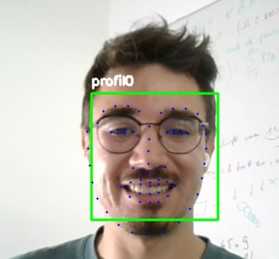
\includegraphics[width=0.5\textwidth]{pictures/68landmarks.jpg}
    \caption{Praxisbeispiel der 68-landmarks}
    \label{fig:68landmarks}
    \cite{68landmarks}
\end{figure}

\subsection{Vergleich der Gesichtsembeddings}
Die erstellten Embeddings werden zur Identifikation von Personen genutzt, indem sie mit bereits gespeicherten Embeddings verglichen werden. \\

\noindent \textbf{Vergleichsmethode}:
Zur Identifikation wird der euklidische Abstand zwischen den Embeddings berechnet. Der euklidische Abstand ist eine Maßzahl für die Distanz zwischen zwei Punkten in einem n-dimensionalen Raum, die durch die Wurzel der Summe der quadrierten Differenzen ihrer Koordinaten berechnet wird. Wenn der Abstand gering ist (unter einem bestimmten Schwellenwert, z.B. 0.6), wird angenommen, dass es sich um dieselbe Person handelt. Der Schwellenwert von 0,6 wurde durch eine Reihe von Tests empirisch bestimmt, um eine Balance zwischen False Positives und False Negatives zu erreichen, was eine zuverlässige Unterscheidung zwischen verschiedenen Personen ermöglichen soll.

\section{Speichern und Verwalten der Profile}

An diesem Zeitpunkt im Projekt war der Kern der Gesichtserkennung, also das Erkennen eines Gesichts, das Erstellen eines Face Embeddings und die Logik für den Vergleich mit bereits erkannten Gesichtern, fertiggestellt. Es folgte also nun die Integration in unser bestehendes System. Die Kommunikation mit dem Display-Webserver lief reibungslos, da dieser auf dem gleichen Gerät gehostet wird und somit nur der Ablagepfad der Profildaten geändert werden musste. Ein größeres Problem war jedoch die Kommunikation mit der Remote-App. Da diese ebenfalls Änderungen an den Profilen vornehmen kann, mussten wir sicherstellen, dass die Profile samt Einstellungen auf beiden Seiten synchron sind, um Informationsverlust oder Schlimmeres zu verhindern. Dafür gab es einige Besprechungen mit dem Entwickler der App, David Vollmer. Wir einigten uns auf ein genormtes Format der Profildatenspeicherung (profiles.json), welches dann über einen Websocket vom Spiegel an die Remote und vice versa gesendet werden kann.
\subsection{Speichern der Profile}
 Wenn ein unbekanntes Gesichtsembedding identifiziert wird, wird ein neues Profil mit Standardwerten in der JSON-Datei erstellt. Diese Datei enthält die Informationen darüber, welche Profile existieren, welches Profil gerade aktiv ist und für jedes Profil, welche Widgets (IDs) an welcher Stelle (index) angezeigt werden sollen. Wird ein Gesichtsembedding wiedererkannt, wird jediglich das dazugehörige 'isSelected' Flag gesetzt und das vorherige gecleared.


\subsection{Verbindung zum Websocket}
Um die Profile mit der Android-Remote zu synchronisieren wurde eine Websocket-Verbindung implementiert. Diese Verbindung ermöglicht die Echtzeitsynchronisation von Profiländerungen zwischen dem Smart Mirror und der Android-App.

\noindent \textbf{Vorgehensweise}:
\begin{itemize}
    \item \textbf{Websocket-Listener}: Sowohl die Remote-App als auch der Smart Mirror haben jeweils einen Listener am Websocket, um Nachrichten zu empfangen.
    
    \item \textbf{Synchronisation beim App-Start}: Beim Starten der Android-App sendet sie einen 'fetch'-Befehl über den Websocket, um sicherzustellen, dass sie sofort mit den aktuellen Profildaten synchronisiert wird. Der Smart Mirror antwortet daraufhin mit der aktuellen profiles.json-Datei.

    \item \textbf{Automatische Updates bei Profiländerungen}: Die profiles.json wird jedes Mal von dem Spiegel an den Websocket gesendet, wenn:
    \begin{itemize}
        \item Ein neues Profil angelegt wurde (das neue Profil erhält automatisch das 'isSelected'-Flag).
        \item Ein neues, aber bereits bekanntes Gesicht erkannt wird und das 'isSelected'-Flag entsprechend gesetzt wurde.
    \end{itemize}

    \item \textbf{Updates von der Remote-App}: Wenn die Remote-App eine Änderung an einem Profil vornimmt, sendet sie die profiles.json an den Websocket. Der Smart Mirror empfängt diese Nachricht und ersetzt die bestehende profiles.json mit den neuen Daten.
\end{itemize}

\section{Schlussfolgerung}



\subsection{Ausblick}
Die Entwicklung der Gesichtserkennungslösung hat eine solide Grundlage geschaffen, auf der zukünftige Erweiterungen und Verbesserungen aufbauen können. Obwohl einige vielversprechende Ideen aufgrund der Stabilität des Systems nicht umgesetzt wurden, bieten sie spannende Möglichkeiten für zukünftige Arbeiten.

\begin{itemize}
    \item \textbf{Age- und Gender-Classifier}: Die Dlib-Bibliothek bietet auch Age- und Gender-Classifier, die in Zusammenarbeit mit dem Widget-Team als eigenständiges Widget hätten angeboten werden können. Lokale Tests hatten dazu bereits funktioniert, und eine vollständige Implementierung könnte die Personalisierung des Smart Mirrors weiter verbessern.
    
    \item \textbf{Änderung des Profilnamens}: Mit mehr Zeit wäre eine Möglichkeit implementiert worden, den Profilnamen zu ändern. Derzeit ist der Profilname der einzigartige Bezeichner für die Face Embeddings. Um dies zu ermöglichen, müsste ein zusätzlicher eindeutiger Bezeichner eingeführt und die Profil-Logik sowohl auf dem Spiegel als auch in der App angepasst werden.
    
    \item \textbf{Flusskontrolle}: Eine weitere wichtige Verbesserung wäre die Einführung einer Flusskontrolle. Derzeit senden Spiegel und App Änderungen sofort, wenn bestimmte Ereignisse auftreten. Dies kann zu Konflikten und inkonsistenten Daten führen, wenn beide Seiten gleichzeitig senden. Eine Flusskontrolle könnte sicherstellen, dass nur eine Seite senden kann, während die andere Seite blockiert ist. Gesendete Änderungen während der Blockierphase würden in einem Puffer gespeichert und nach der Blockierung sofort gesendet.
    
    \item \textbf{Optimierung des Schwellenwerts}: Mit mehr Zeit hätten intensivere Tests zur Einstellung des euklidischen Abstands durchgeführt werden können, um Fehler wie bei der Produktpräsentation zu vermeiden. Ein genauer kalibrierter Schwellenwert könnte die Erkennungsgenauigkeit weiter verbessern und sicherstellen, dass neue Gesichter nicht fälschlicherweise als bekannte Profile erkannt werden.
    
    \item \textbf{Datenbanksynchronisation}: Wenn wir vorher gewusst hätten, wie aufwändig die Synchronisation der Profile sein würde, hätten wir definitiv eine Datenbank verwendet , die die Synchronisation eigenständig durchführt. Eine Datenbank könnte viele der aktuellen Herausforderungen bei der Datenkonsistenz und -synchronisation lösen.
\end{itemize}

\subsection{Zusammenfassung}
Im Verlauf dieses Projekts wurde eine fortschrittliche Gesichtserkennungslösung für einen Smart Mirror entwickelt. Der Übergang von herkömmlichen Haar-Cascades zu modernen Methoden wie Dlib und HOG führte zu einer signifikanten Verbesserung der Erkennungsgenauigkeit. Trotz der Performance-Probleme konnte eine zufriedenstellende Verarbeitungsgeschwindigkeit erreicht werden.

\noindent Ein wichtiger Teil des Projekts war die Speicherung und Verwaltung der Profildaten sowie die Synchronisation mit einer Android-Remote-App über eine Websocket-Verbindung. Die Trennung der Face Embeddings von der profiles.json-Datei und die Implementierung eines robusten Synchronisationsmechanismus stellten sicher, dass die Daten auf beiden Seiten konsistent und aktuell blieben.

\noindent Insgesamt konnte eine zuverlässige Gesichtserkennung und Profilverwaltung implementiert werden.


\chapter{Schnittstelle}

In diesem Kapitel wird die Schnittstelle des \textbf{Spiegel AI} Projekts beschrieben. Wir erläutern die verschiedenen Schnittstellen, die verwendet werden, sowie deren Implementierung und Nutzung.

\section{Überblick}
Geben Sie einen Überblick über die verwendeten Schnittstellen.

\section{Implementierung}
Beschreiben Sie die Implementierung der Schnittstellen.

\section{Nutzung}
Erläutern Sie, wie die Schnittstellen genutzt werden.

\subsection{Dynamische Widget Anordnung}
Erarbeitet von: Marcel Wagner \\ \\
Die Entwicklung eines Smart Mirrors mit dynamisch anpassbarer Display Anordnung stellt eine technische Herausforderung dar. Das Ziel dieses Bereiches war es, eine benutzerfreundliche und flexible Oberfläche zu schaffen, die sich den individuellen Präferenzen der Benutzer anpasst. Dieser Abschnitt beschreibt ausführlich die Methodik der Implementierung der dynamischen Display Anordnung sowie die dabei aufgetretenen Probleme und deren Lösungen. \\ \\
Ein essenzieller Bestandteil des Systems war die kontinuierliche Überwachung der 'profiles.json' Datei. Diese Datei wird von der Gesichtserkennung erstellt. Auf diesen Bereich wurde im vorherigen Kapitel bereits eingegangen. Hierzu wurde ein periodischer Abrufmechanismus implementiert, der alle 200 Millisekunden die Datei abfragt. Bei jeder Abfrage wurde der aktuelle Inhalt der Datei mit dem vorherigen Zustand verglichen, um Änderungen zu erkennen. Diese Methode stellte sicher, dass Anpassungen in den Benutzerprofilen zeitnah detektiert und umgesetzt wurden. \\ \\
Aus dieser Datei wird beginnend nach dem aktuellen ausgewählten Profil gesucht. Zur Identifikation des aktuell ausgewählten Profils wurde eine spezielle Funktion entwickelt. Diese Funktion durchsuchte die Liste der Profile nach dem als ausgewählt markierten Profil und gibt diese zurück. Ist kein Profil ausgewählt, wird null zurückgegeben, was die Anwendung des Standardzustands bedeutet. Die Fähigkeit, das aktive Profil zu identifizieren, war entscheidend für die Anpassung der Display Anordnung und stellte sicher, dass die Benutzereinstellungen korrekt umgesetzt wurden. \\ \\
Als nächster Schritt war ein weiterer zentraler Aspekt der Implementierung eine Funktion für die Ermittlung des aktuellen Zustands der Widgets. Hierbei wird das vorher ausgelesene Profil genutzt um hierfür den Zustand und Positionierung der Widgets auszulesen. Diese flexible Handhabung ermöglichte es, die Anzeige dynamisch an die individuellen Präferenzen der Benutzer anzupassen. \\ \\
Abschließend mussten noch auf Basis dieser Daten eine Dynamische Anpassung der HTML Seite vorgenommen werden.  Basierend auf dem aktuellen Zustand der Widgets wurden die entsprechenden HTML Elemente ein- oder ausgeblendet und in der gewünschten Reihenfolge angeordnet. Diese Anpassungen wurden durch die Funktion 'updateState' gesteuert, die die Widgets gemäß den Benutzereinstellungen neu positionierte. Die Funktion arbeitete folgendermaßen: Zunächst wird der Container, der die Widgets enthielt, geleert. Anschließend werden die Widgets gemäß der im Profil definierten Reihenfolge wieder hinzugefügt. Dabei wird auch die Sichtbarkeit jedes Widgets entsprechend dem enabled Status beachtet. Widgets, die nicht aktiviert waren, werden ausgeblendet, während aktivierte Widgets sichtbar blieben. Diese dynamische Anpassung ermöglichte es, die Widgets je nach Benutzerprofil in der gewünschten Anordnung und Sichtbarkeit darzustellen.

\subsection*{Aufgetretene Probleme und deren Lösung}
\textbf{Cache Verwaltung:} Das am häufigsten aufgetretene Problem war das der Cache Verwaltung des Browsers. Dies stellte eine besondere Herausforderung dar, da durch die regelmäßigen Anfragen an die 'profiles.json' Datei oft veralteter Inhalt aus dem Cache verwendet wurde, anstatt die neuesten Daten abzurufen. Dieses Problem wurde durch gezielte Deaktivierung des Caches für die betreffenden Anfragen gelöst. Der HTTP Header Cache Control wurde entsprechend konfiguriert, um sicherzustellen, dass die Anfragen stets frische Daten zurückliefert. Dies gewährleistete, dass immer die aktuellste Version der profiles.json Datei abgerufen und verarbeitet wurde, was eine zuverlässige Aktualisierung der Anzeige ermöglicht. \\ \\
\noindent
\textbf{CORS Beschränkung:} Ein weiteres Problem, welches während der Implementierung aufgetreten ist, war im Zusammenhang mit der Same Origin Policy des Browsers. Diese Sicherheitsrichtlinie verhinderte den Abruf der profiles.json Datei von einem anderen Ursprung, was die Aktualisierung der Profile erschwerte. Um dieses Problem zu umgehen, wurde ein lokaler Server mit Python erstellt, der die Datei ausliefert. Dieser Server ermöglichte es, die Datei lokal zu hosten und somit die CORS Beschränkungen (Cross Origin Resource Sharing) zu umgehen. Durch den Zugriff auf diesen lokalen Server konnte die Datei problemlos und sicher abgerufen werden, was die zuverlässige Aktualisierung der Profile gewährleistet.
\\ \\
\noindent
\textbf{Fehler bei der Skript ausführung:} Während der Implementierung der Dynamischen Widget Anordnung trat ein weitere Fehler auf, der verhinderte, dass das Skript in der 'updateState.js' Datei ausgeführt wurde. Um das Problem zu beheben war es für mich notwendig das Skript manuell in den code auszuführen. \\ \\
Durch diese manuelle Einbindung konnte der Fehler erfolgreich behoben und die korrekte Funktion des Skriptes sichergestellt werden. Diese Fehlerbehebung war notwendig um den weiteren Verlauf der Widget Anordnung zu gewährleisten.



\chapter{Ergebnisse}

In diesem Kapitel fassen wir die Ergebnisse des Projekts \textbf{Spiegel AI} zusammen. Wir gehen auf die erreichten Ziele, die Herausforderungen und die zukünftigen Arbeiten ein.

\section{Zusammenfassung der Ergebnisse}

\subsection{Erreichte Ziele}
Unser Projektteam hat den Smart Mirror erfolgreich realisiert und dabei folgende Ziele erreicht:

Der Spiegelprototyp wurde ansehnlich und robust aufgebaut. Er ist nicht nur funktional, sondern fügt sich auch optisch ansprechend in die Umgebung ein. Die Display-Ausgabe funktioniert einwandfrei und ermöglicht eine klare und deutliche Darstellung aller Inhalte.

Der Smart Mirror ist in der Lage, die aktuelle Wetterlage des Ortes sowie Kalendereinträge anzuzeigen und bietet viele weitere informative und nützliche Funktionen. Benutzer des Spiegels haben die Möglichkeit, ihr angezeigtes Profil individuell zu gestalten. Dies erfolgt durch die Auswahl aus neun verschiedenen Widgets, die auf acht unterschiedlichen Positionen platziert werden können. Diese Personalisierung ermöglicht eine hohe Flexibilität und Anpassungsfähigkeit an die individuellen Bedürfnisse und Vorlieben der Benutzer.

Ein weiteres herausragendes Merkmal ist die interaktive Steuerung über eine mobile Kontroll-App. Diese App ermöglicht es den Benutzern, ihr Profil zu ändern oder zu personalisieren, was die Benutzerfreundlichkeit und den Komfort erheblich steigert. Alle Informationen werden in deutscher Sprache angezeigt, was die Bedienung für deutschsprachige Nutzer intuitiv und einfach macht.

Ein neues Gesicht wird erkannt und das jeweilige Profil angezeigt, was eine schnelle und reibungslose Nutzung sicherstellt. Die Benutzeroberfläche wurde in Tests als 'sehr intuitiv' eingestuft, was die hohe Benutzerfreundlichkeit des Systems unterstreicht.

Technisch konnten wir sicherstellen, dass sowohl der Spiegel als auch die App erfolgreich eine Verbindung zum Websocket herstellen können. Beide Komponenten senden nach einer ausgeklügelten Synchronisationslogik jeweils den aktuellen Stand der Profile, wodurch eine konsistente und aktuelle Datenbasis gewährleistet wird. Die Gesichtserkennung arbeitet äußerst zuverlässig und erkennt Personen zu 95 Prozent korrekt, wodurch die personalisierten Profile geladen und angezeigt werden können.

\subsection{Herausforderungen}
Die Herausforderungen, denen sich das Team während der Entwicklung des Projekts stellen musste, sind in den jeweiligen Dokumentationen der einzelnen Projektteilnehmer ausführlich beschrieben. 

\subsection{Zukünftige Arbeiten}
Für zukünftige Arbeiten und mögliche Erweiterungen des Projekts verweisen wir ebenfalls auf die detaillierten Ausführungen in den Dokumentationen der einzelnen Projektteilnehmer.


\chapter*{Stundenliste}
\addcontentsline{toc}{chapter}{Stundenliste}

\begin{longtable}[c]{|c|>{\raggedright\arraybackslash}p{2.5cm}|>{\raggedright\arraybackslash}p{7cm}|}
\caption*{\textbf{Stundenliste Leon Kranner}} \\
\hline
\textbf{Kalenderwoche} & \textbf{Stunden} & \textbf{Aufgabe} \\
\hline
\endfirsthead

\multicolumn{3}{c}%
{\tablename\ \thetable{} -- Fortsetzung von vorheriger Seite} \\
\hline
\textbf{Kalenderwoche} & \textbf{Stunden} & \textbf{Aufgabe} \\
\hline
\endhead

\hline \multicolumn{3}{r}{{Fortsetzung auf nächster Seite}} \\
\endfoot

\hline
\endlastfoot

12 & 3 & Einführungsveranstaltung \\
     & 3 Requirements + Materialliste \\
\hline
13 & 3 & GANNT Diagramm \\
   & 2 & Teambesprechung \\
\hline
14 & 2 & Planung mit Hardware-Team \\
   & 2 & Teambesprechung \\
   & 1 & Requirements überarbeiten \\
   & 3 & Planung Produkterstellung \\
\hline
15 & 3 & Postererstellung und Hw \\
   & 2 & Displaymessung + Postervorstellung \\
   & 2 & Teambesprechung \\
   & 1 & Baumarkt \\
   & 2 & Besprechung Spiegelrahmen \\
\hline
16 & 4 & Display-Projekt aufsetzen \\
    & 2 & Baumarkt Materialien erkunden \\
    & 2 & Planung/Besprechung Bilderrahmen \\
    & 2 & Teambesprechung \\ 
\hline
17 & 2 & Umstrukturierung des Display-Projekts \\
   & 2 & Neues Widget erstellen \\
    & 3 & Projektbesprechung und weitere Programmierung \\
    & 2 & Teambesprechung \\
\hline
18 & 6 & Weitere Widgets und Änderungen an alten Widget \\
     & 2 & Bugfixing beim Kalender \\
     & 4 & Holz auf Maß schneiden und hobeln \\
     & 3 & Vorbohren und Bilderrahmen zurechtlegen \\ 
\hline
19 & 3 & Einkerbungen fräsen \\
    & 1 & MDF Platte auf Maß schneiden \\
    & 1 & Zwischenstücke vorne anschrauben \\
    & 1 &  Teambesprechung \\
    & 2 & Holz zusammenleimen und trocknen lassen \\
\hline
20 & 2 & Teambesprechung \\
    & 1 & Umstrukturierung des Stundenplans \\
\hline
21 & 2 & Teambesprechung \\
     & 1 & Plexiglas auf Maß schneiden \\
\hline
22 & 2 & Teambesprechung \\
     & 7 & Display dynamisch gestalten + Automatische Aktualisierung der Widgets \\
\hline
23 & 2 & Automatische Aktualisierung der Widgets \\
     & 2 & Teambesprechung \\
\hline
24 & 2 & Teambesprechung \\
   & 2 & Besprechung Schnittstellen \\
    & 2 & Bugfixing Kalender Widget (Anzeigen des aktuellen Tages) \\
\hline
25 & 2 & Teambesprechung \\
   & 1 & Plexiglas überarbeiten \\
   & 2 & Löcher bohren und Plexiglas festschrauben \\
   & 1 & Spiegelfolie aufbringen und Kabel-Loch bohren \\
   & 3 & Fine tuning für Display (Anpassung Widget: Größe, Formatierung, Anordnung, etc.) \\
   & 3 & Aufbau und Testen des Displays \\
\hline
26 & 2 & Teambesprechung \\
     & 1 & Fehler korrigieren am Spiegel \\
   & 3 & Austausch der Spiegel Folie, Aufbau der Spiegels, Hardware installieren \\
   & 1 & Testen des Displays mit Aufgebauten Spiegels \\
   & 1 & Besprechung Präsentation \\
   & 2 & Vorbereitung Präsentation Bilder und Aufbau \\
   & 2 & Raspberry Pi Gesichtserkennung testen \\
   & 1 & Anpassung des Kalenders: Monate nebeneinander anzeigen statt untereinander \\
   & 1 & Anpassung der Wettervorhersage: nur 3 Tage und nicht untereinander \\
\hline
27 & 2 &  Powerpoint vorbereiten \\
     & 1 & Text für Präsentation vorbereiten \\
     & 1 & Vorbereitung Präsentation \\
     & 3 & Final Version von Projekt auf Raspberry spielen + Testen aller Funktionen \\
     & 2 & Teambesprechung \\
     & 1 & Stundenliste in Dokumentation eintragen \\
     & 2 & Informieren über Mögliche Testvarianten für Widget \\     
     & 1 & Einleitung der Dokumentation schreiben \\
     & 3 & Verschieden Testvarianten bei den Widgets durchführen \\

\hline
28 & 2 & Dokumentation für Hardware schreiben \\
     & 3 & Dokumentation für Widgets \\
     & 3 & Dokumentation für Rahmen \\
     & 2 & Dokumentation für Display-Aufbau schreiben + Kapitel formatieren in Latex\\
     & 1 & Testverfahren für Doku schreiben
\end{longtable}

Gesamtstunden: 148

% Neue Seite für die nächste Tabelle
\newpage


\begin{longtable}[c]{|c|>{\raggedright\arraybackslash}p{2.5cm}|>{\raggedright\arraybackslash}p{7cm}|}
\caption*{\textbf{Stundenliste Marco Kuner}} \\
\hline
\textbf{Kalenderwoche} & \textbf{Stunden} & \textbf{Aufgabe} \\
\hline
\endfirsthead

\multicolumn{3}{c}%
{\tablename\ \thetable{} -- Fortsetzung von vorheriger Seite} \\
\hline
\textbf{Kalenderwoche} & \textbf{Stunden} & \textbf{Aufgabe} \\
\hline
\endhead

\hline \multicolumn{3}{r}{{Fortsetzung auf nächster Seite}} \\
\endfoot

\hline
\endlastfoot

12 & 3 & Einführungfsveranstaltung \\
\hline
13 & 3 & GANNT Diagramm \\
\hline
14 & 3 & Teileliste / GANNT Diagramm \\
   & 2 & Teambesprechung \\
   & 3 & Inventur \\
\hline
15 & 10 & Technologie-Recherche + Postererstellung \\
   & 3 & Posterdemütigung ertragen und HW \\
   & 2 & Teambesprechung \\
\hline
16 & 2 & Teambesprechung \\
   & 8 & Erster Prototyp mit HAAR Cascades \\
\hline
17 & 2 & Teambesprechung \\
   & 8 & Neue Version mit DLIB Bibs geschrieben \\
\hline
18 & 2 & Teambesprechung \\
   & 2 & Recherche über facial Landmark Storage \\
   & 4 & Neue Iteration mit Storage Technologie \\
\hline
19 & 10 & Troubleshoot da extrem langsam \\
   & 2 & Teambesprechung \\
\hline
20 & 2 & Teambesprechung \\
   & 4 & Recherche zu geeigneter Schnittstelle und Format der Profilerstellung mit profile landsmarks \\
\hline
21 & 2 & Teambesprechung \\
\hline
22 & 2 & Teambesprechung \\
\hline
23 & 2 & Teambesprechung \\
\hline
24 & 2 & Teambesprechung \\
\hline
25 & 2 & Teambesprechung \\
   & 6 & Implementieren einer Lösung zur automatischen Erkennung eines neuen Gesichts und output der Daten in .json \\
   & 2 & Schnittstellen Thinktank mit David \\
\hline
26 & 2 & Teambesprechung \\
   & 5 & Ausgabe und automatische Aktualisierung einer genormten profiles.json \\
   & 6 & Implementierung eines neuen Websockets zwischen Raspi und Android in Vorbereitung zur Synchronisation \\
   & 2 & Recherche zu Technologien zur Synchronisation zwischen Raspi und Android (inotify?) \\
   & 2 & Besprechung mit remote app Spezialist bzgl. Synchronisationsproblemen \\
\hline
27 & 4 & Vor- und Aufbereiten der Präsentation \\
   & 2 & Verbessern der readability des Algorithmus \\
   & 8 & Implementation des Websockets mitsamt Logik für andauernder Synchronisation \\
   & 4 & Troubleshooting: Gesichtserkennung stürzt ab auf Raspi \\
   & 3 & Testing \\
   & 6 & Dokumentation Gesichtserkennung  \\
   & 3 & Literatur+Abbildungsverzeichnis\\
\end{longtable}

Gesamtstunden: 140

% Neue Seite für die nächste Tabelle
\newpage


\begin{longtable}[c]{|c|>{\raggedright\arraybackslash}p{2.5cm}|>{\raggedright\arraybackslash}p{7cm}|}
\caption*{\textbf{Stundenliste David Vollmer}} \\
\hline
\textbf{Kalenderwoche} & \textbf{Stunden} & \textbf{Aufgabe} \\
\hline
\endfirsthead

\multicolumn{3}{c}%
{\tablename\ \thetable{} -- Fortsetzung von vorheriger Seite} \\
\hline
\textbf{Kalenderwoche} & \textbf{Stunden} & \textbf{Aufgabe} \\
\hline
\endhead

\hline \multicolumn{3}{r}{{Fortsetzung auf nächster Seite}} \\
\endfoot

\hline
\endlastfoot

12 & 3 & Einführungsveranstaltung \\
   & 4 & Setup Gitlab und Drafts \\
\hline
13 & 4 & Erstellung GANNT Diagramm und Lastenheft \\
   & 2 & Teambesprechung \\
\hline
14 & 5 & Abgabevorbereitung GANNT und Lastenheft \\
   & 2 & Teambesprechung \\
   & 3 & Hardwarediskussion und -suche \\
   & 2 & Überarbeitung GANNT und Lastenheft \\
\hline
15 & 4 & Postererstellung \\
   & 3 & Vostellung Poster und Hardwaresuche \\
   & 6 & Setup Flutter und Frontend dev \\
   & 2 & Teambesprechung \\
   & 2 & Frontend dev (Navigation) \\
\hline
16 & 2 & Teambesprechung \\
   & 3 & Frontend dev \\
\hline
17 & 2 & Setup Raspberry Pi \\
   & 2 & Teambesprechung \\
\hline
18 & 2 & Teambesprechung \\
\hline
19 & 2 & Teambesprechung \\
   & 1 & Frontend dev (Widget buttons) \\
\hline
20 & 2 & Teambesprechung \\
\hline
21 & 2 & Teambesprechung \\
\hline
22 & 2 & Teambesprechung \\
   & 4 & Troubleshooting Android SDK \\
\hline
23 & 2 & Teambesprechung \\
\hline
24 & 2 & Besprechung Schnittstellen \\
   & 4 & Frontend dev (Widgets final) \\
   & 2 & Teambesprechung \\
   & 2 & Konfiguration Raspberry Pi \\
   & 8 & Konfiguration Schnittstellen (Flutter + Server) \\
   & 5 & Konfiguration Schnittstellen (Spiegel + Server) \\
\hline
25 & 2 & Teambesprechung \\
   & 3 & Konfiguration Raspberry Pi wifi \\
   & 5 & Troubleshooting + Testing Websocket \\
   & 2 & Anpassung Android und iOS (icon, splash, usw.) \\
   & 8 & Anpassung Datenspeicher, Profile und Websocket \\
   & 3 & Speichern von Widget- und Remotestatus in Profilen \\
   & 3 & Code Refactoring und Bugfixing \\
\hline
26 & 1 & Besprechung Schnittstellen Profile \\
   & 1 & Überarbeitung Poster \\
   & 2 & Teambesprechung \\
   & 1 & Überarbeitung Websocket-Message \\
   & 2 & Troubleshooting selected Widgets \\
   & 2 & Konfiguration Raspberry Pi Gesichtserkennung \\
   & 6 & Erstellung Powerpoint \\
\hline
27 & 2 & Besprechung profiles sync \\
   & 1 & Refactoring File Reader \\
   & 2 & Implementierung profiles sync \\
   & 3 & Schreiben des Präsentationsskripts \\
   & 2 & Übung Präsentation \\
   & 5 & Testen der Gesichtserkennung am Websocket \\
   & 4 & Testen und Korrigieren profiles sync \\
   & 2 & Überarbeitung Dokumentationslayout \\
   & 5 & Implementierung und Testen selectedWidgets \\
   & 1 & Kompilieren Remote App Release \\
   & 2 & Dokumentation Remote App Views \\
   & 2 & Anpassung des Literaturverzeichnisses in Dokumentation \\
   & 1 & Dokumentation Flutter SDK \\
   & 2 & Dokumentation Implementierung Websocket und Remote Content \\  
\hline
28 & 2 & Dokumentation Raspberry Pi Konfiguration \\
   & 3 & Dokumentation Implementierung Widgets, Profile und Sonstiges \\
   & 2 & Dokumentation Schnittstellen \\
   & 1 & Dokumentation Fertigstellung \\
\end{longtable}

Gesamtstunden: 174

% Neue Seite für die nächste Tabelle
\newpage

\begin{longtable}[c]{|c|>{\raggedright\arraybackslash}p{2.5cm}|>{\raggedright\arraybackslash}p{7cm}|}
\caption*{\textbf{Stundenliste Marcel Wagner}} \\
\hline
\textbf{Kalenderwoche} & \textbf{Stunden} & \textbf{Aufgabe} \\
\hline
\endfirsthead

\multicolumn{3}{c}%
{\tablename\ \thetable{} -- Fortsetzung von vorheriger Seite} \\
\hline
\textbf{Kalenderwoche} & \textbf{Stunden} & \textbf{Aufgabe} \\
\hline
\endhead

\hline \multicolumn{3}{r}{{Fortsetzung auf nächster Seite}} \\
\endfoot

\hline
\endlastfoot

12 & 3 & Einführungfsveranstaltung \\
\hline
13 & 3 & GANNT Diagramm \\
   & 2 & Teambesprechung \\
   & 2 & Vorbereitung Template \\
\hline
14 & 2 & Teambesprechung \\
   & 3 & Planung und Hardware Suche \\
   & 3 & Setup CAD und ersten Entwurf zeichnen \\
\hline
15 & 3 & Poster Erstellung \\
   & 2 & Besprechung Spiegelrahmen \\
   & 2 & Detaillierung der CAD Datei \\
   & 1 & Baumarkt \\
   & 2 & Teambesprechung \\
\hline
16 & 3 & Einführung Display Programmierung und erste Ansätze \\
   & 2 & Planung und Besprechung für den Bilderrahmen \\
   & 2 & Materialien im Baumarkt suchen \\
   & 2 & Teambesprechung \\
\hline
17 & 4 & Weitere Setup für Display Programmierung \\
   & 4 & Projekt Besprechung und weitere Programmierung \\
   & 4 & Weitere Widget Programmierung und Bug Fixing \\
   & 2 & Teambesprechung \\
\hline
18 & 2 & Display Programmierung (Fertigstellung des Verkehrsinformations Widget) \\
   & 2 & Teambesprechung \\
   & 4 & Holz auf Maß schneiden und hobeln \\
   & 3 & Vorbohren und Bilderrahmen zurechtlegen \\
\hline
19 & 3 & Einkerbungen fräsen \\
   & 1 & MDF Platte auf Maß schneiden \\
   & 1 & In MDF Platte Löcher bohren für Befestigung \\
   & 1 & Zwischenstücke vorne anschrauben \\
   & 2 & Teambespechung \\
   & 2 & Holz zusammenleimen und trocknen lassen \\
\hline
20 & 2 & Teambesprechung \\
   & 1 & Bug Fixing von älteren Widgets \\
\hline
21 & 2 & Teambesprechung \\
   & 1 & Plexiglas auf Maß schneiden \\
\hline
22 & 2 & Teambesprechung \\
\hline
23 & 3 & Erstellung weiter Widgets \\
   & 2 & Teambespechung \\
\hline
24 & 2 & Teambesprechung \\
   & 2 & Besprechung Schnittstellen \\
   & 2 & Bugfixing für das News Widget \\
\hline
25 & 2 & Teambesprechung \\
   & 1 & Bugfixing der Widget Ansicht \\
   & 1 & Plexiglas überarbeiten \\
   & 2 & Löcher bohren und Plexiglas festschrauben \\
   & 1 & Spiegelfolie aufbringen und Kabel Loch bohren \\
   & 5 & Schnittstelle zwischen Gesichtserkennung und Display die Grundlagen auf Seite des Displays aufsetzen \\
   & 2 & Bugfixing Schnittstellen Problem\\
\hline
26 & 2 & Teambesprechung \\
   & 1 & Fehler korrigieren am Spiegel \\
   & 1 & Bugfixing Widget \\
   & 3 & Austausch der Spiegel Folie, Aufbau der Spiegels, Hardware installieren \\
   & 1 & Testen des Displays mit Aufgebauten Spiegels \\
   & 1 & Vorbereitung Präsentation \\
   & 2 & Vorbereitung Präsentation (Bilder und Aufbau Finalisieren) \\
   & 2 & Raspberry Pi Gesichtserkennung Testen \\
   & 5 & Profile aus der Gesichtserkennung auslesen und Speicherin in Raspberry \\
   & 2 & Bugfixing Browser Problem \\
\hline
27 & 2 & Powerpoint erstellung \\
   & 3 & HMTL neu anordnen auf Basis von Json Datei\\
   & 2 & Troubleshooting Cache Probleme \\
   & 1 & nicht ausgewählte Widgets ausblenden \\
   & 2 & Vorbereitung Präsentation \\
   & 3 & Schreiben des Präsentationsskripts \\
   & 2 & Teambespechung \\
   & 1 & Studenliste in Dokumentation eintragen \\
   & 4 & Dokumentation für Widgets schreiben \\
   & 1 & Dokumentation für Testverfahren schreiben \\
   & 2 & Informieren über Mögliche Testvarianten für Widget / Schnittstelle \\
   & 3 & Verschieden Testvarianten bei den Widgets durchführen \\
   & 2 & Dokumentation der Dynamischen Widget Anordnung / Überarbeitung Layout \\
   & 2 & Dokumentation für Hardware schreiben \\
   & 3 & Dokumentation für Rahmen \\
   & 1 & Quellen aktualisieren und kleine Fehlerbehebungen in der Dokumentation \\
   & 3 & Final Version von Projekt auf Raspberry spielen und Testen aller Funktionen für die Vorstellung \\
\hline
28 & 1 &  Dokumentation der Fehler bei der Implementierung der Dynamischen Widget anordnung \\
   & 1 & Korrektur der Fertigen Dokumentation \\

\end{longtable}

Gesamtstunden: 166

\newpage

\chapter*{Literaturverzeichnis}

\printbibliography[heading=none]

\listoffigures

\end{document}
